From the PAMPA and Caco-2 assays performed by our collaborators, a large ``permeability cliff''  between Nleu-5R and 5S could be identified (Figure \ref{fig:permAssays}). Permeability cliffs were also observed between some other pairs of epimers, but to a lesser extent (e.g., Nala-4R vs 4S with $−log(P_e)$~=~$7.6$ and $6.6$, Nphe-2R vs 2S with $−log(P_e)$~=~$7.2$ and $6.3$, and Nphe-3R vs 3S with $−log(P_e)$~=~$7.5$ and $6.5$). 
Extensive MD simulations were carried out in a polar and apolar environment (i.e., water and chloroform) to study the influence of the stereocenter change on the conformational behavior of the molecules. As a negative control group, we used the molecule pair Nleu-2R and 2S. 

\FloatBarrier
%-------------------------------------------

\subsection{Starting Configurations} 
The starting conformations used for the MD simulations were generated with the macrocycle variant of the OMEGA conformer generator from OpenEye.  \cite{Hawkins2012, Hawkins2010, Poongavanam2018}
The generated conformers showed similar distributions in terms of hydrogen bonds (H-bonds) and backbone torsional angles for the enantiomer pairs (Tables \ref{tab: SIhbondRatios} and \ref{tab: SIhbondAmountRatios}).
Therefore, we started the MD simulations for each enantiomer pair from similar starting points.
In these conformer ensembles, approximately $50\%$ of the structures had a trans-peptoid bond for each molecule, and $50\%$ had a cis-peptoid bond.

\begin{table}[h!]
\centering
\caption{Hydrogen-bond occurrence in percentage for the starting conformations of Nleu-5R, Nleu-5S, Nleu-2R, and Nleu-2S.}
\label{tab: SIhbondRatios}
  \begin{adjustbox}{max width=\textwidth}
  \begin{tabular}{lcccc}
Hydrogen bond {[}\%{]} & Nleu-2R      & Nleu-2S      & Nleu-5R      & Nleu-5S      \\
\hline
NLEU-O tether-NH       & 14         & 15         &  9           & 9        \\
ALA-O tether NH        & \textless{}1 & \textless{}1  & \textless{}1  & \textless{}1 \\
PHE-O Ala-NH           & \textless{}1 & \textless{}1 & \textless{}1  & \textless{}1 \\
ALA-O PHE-NH           & 24           & 7            & 21 & 19 \\
    \hline
\end{tabular}%
\end{adjustbox}
\end{table}


\begin{table}[h!]
\centering
\caption{Percentage of starting conformations with zero, one, or two hydrogen bonds for
Nleu-5R, Nleu-5S, Nleu-2R, and Nleu-2S.}
\label{tab: SIhbondAmountRatios}
  \begin{adjustbox}{max width=\textwidth}
\begin{tabular}{llll}
Hydrogen bond {[}\%{]} & 0      & 1          & 2        \\
    \hline
Nleu-2R        & 36             & 52         &  1       \\
Nleu-2s        & 39             & 51         &  1       \\
Nleu-5R        & 34             & 52         &  13      \\
Nleu-5S        & 37             & 51         &  12  \\
   \hline

\end{tabular}%
\end{adjustbox}
\end{table}

\FloatBarrier
%-------------------------------------------

\subsection{CNN Clustering} 
The cumulative 25~$\mu$s simulation data for each peptide and solvent were clustered separately based on the backbone dihedrals and the polar atom distances. The resulting clusters could be structurally classified depending on the conformation of the peptoid bond (i.e., cis or trans; see Tables \ref{tab:SIClusterTransCHCL3} and \ref{tab: SIClusterTransWater}). The number of generated clusters varied but usually the size of the clusters decreased rapidly. Conformations with a cis or trans-peptoid bond were cleanly separated into different clusters.

\begin{table}[h!]
\center
\caption{List of clusters identified in the simulations in chloroform with the  respective population (in percentage). Clusters with the peptoid bond in trans-conformation are labeled with *. In the other clusters, the peptoid bond is in cis-conformation.}
\label{tab:SIClusterTransCHCL3}
  \begin{adjustbox}{max width=\textwidth}
\begin{tabular}{c|lc||c|lc}
Molecule                  & Cluster & Size $[\%]$ & Molecule                  & Cluster & Size $[\%]$ \\
\hline
\multirow{11}{*}{NLeu-5R} & 1*      & 36.2        & \multirow{11}{*}{NLeu-5S} & 1*      & 41.0        \\
                          & 2       & 18..1       &                           & 2       & 16.0        \\
                          & 3       & 16.1        &                           & 3       & 9.2         \\
                          & 4*      & 15.4        &                           & 4       & 7.4         \\
                          & 5       & 3.5         &                           & 5*      & 6.6         \\
                          & 6       & 1.5         &                           & 6*      & 0.6         \\
                          & 7       & 0.5         &                           & 7       & 0.6         \\
                          & 8       & 0.3         &                           & 8       & 0.2         \\
                          & 9       & 0.2         &                           & 9       & 0.2         \\
                          & Noise   & 8.2         &                           & 10      & 0.1         \\
                          &         &             &                           & Noise   & 18.0        \\
\hline
\multirow{6}{*}{Nleu-2R}  & 1*      & 53.3        & \multirow{13}{*}{Nleu-2S} & 1*      & 26.2        \\
                          & 2       & 17.6        &                           & 2*      & 18.3        \\
                          & 3       & 11.7        &                           & 3       & 15.7        \\
                          & 4       & 10.2        &                           & 4       & 6.5         \\
                          & 5       & 2.8         &                           & 5       & 6.3         \\
                          & Noise   & 4.4         &                           & 6       & 5.2         \\
                          &         &             &                           & 7*      & 5.1         \\
                          &         &             &                           & 8       & 1.3         \\
                          &         &             &                           & 9*      & 0.6         \\
                          &         &             &                           & 10*     & 0.5         \\
                          &         &             &                           & 11      & 0.3         \\
                          &         &             &                           & 12*     & 0.3         \\
                          &         &             &                           & Noise   & 13.0       
\end{tabular}%
\end{adjustbox}
\end{table}

%SI-tab: 10
\begin{table}[h!]
\center
\caption{ List  of  clusters  identified  in  the  simulations  in  water  with  the  respective 
population  (in  percentage).  Clusters  with  the  peptoid  bond  in  trans-conformation  are 
labeled with *. In the other clusters, the peptoid bond is in cis-conformation}
\label{tab: SIClusterTransWater}
  \begin{adjustbox}{max width=\textwidth}
\begin{tabular}{c|lc||c|lc}
Molecule                  & Cluster & Size $[\%]$ & Molecule                  & Cluster & Size $[\%]$ \\
\hline
\multirow{11}{*}{NLeu-5R} & 1*      & 46.7        & \multirow{11}{*}{NLeu-5S} & 1*      & 51.3        \\
                          & 2       & 22.4       &                            & 2       & 16.8        \\
                          & 3       & 20.8        &                           & 3       & 8.7         \\
                          & 4       & 6.1        &                            & 4       & 8.0         \\
                          & 5       & 1.5        &                            & 5       & 3.7         \\
                          & 6*      & 0.6         &                           & 6       & 3.6         \\
                          & 7       & 0.4         &                           & 7       & 1.7         \\
                          & 8*      & 0.4         &                           & 8*      & 1.7         \\
                          & 9*      & 0.2         &                           & 9*      & 0.8         \\
                          & Noise   & 1.0         &                           & 10      & 0.4         \\
                          &         &             &                           & 11*     & 0.2         \\
                          &         &             &                           & Noise   & 3.2        \\
\hline
\multirow{6}{*}{Nleu-2R}  & 1*      & 50.2        & \multirow{13}{*}{Nleu-2S} & 1*      & 42.0        \\
                          & 2       & 21.0        &                           & 2       & 19.0        \\
                          & 3       &  6.6        &                           & 3       & 12.0        \\
                          & 4       &  5.6        &                           & 4       &  7.7        \\
                          & 5       &  4.7        &                           & 5       &  6.3        \\
                          & 6       &  2.6        &                           & 6       &  3.5     \\
                          & 7       &  1.6        &                           & 7       &  2.7        \\
                          & Noise   &  7.8        &                           & 8*      &  1.4        \\
                          &         &             &                           & 9*      &  0.1        \\
                          &         &             &                           & Noise   &  5.0       
\end{tabular}%
\end{adjustbox}
\end{table}


The cis-trans isomerization represents a very slow process in the simulations, which occurred only rarely (Table \ref{tab: SICisTransTrans}). Due to the low number of transitions, the process could not be modeled robustly. Therefore, the clusters with the cis- and trans-peptoid bond are analyzed separately in the following.
\begin{table}[h!]
\centering
\caption{ Occurrence  of  cis-trans  isomerization  of  the  peptoid  bond  during  the  MD 
simulations (25 μs in water and chloroform, respectively}
\label{tab: SICisTransTrans}
\begin{adjustbox}{max width=\textwidth}
\begin{tabular}{r|cc|cc}
\multirow{2}{*}{Molecule} & \multicolumn{2}{l}{Chloroform} & \multicolumn{2}{|l}{Water}        \\
    & Cis \rightarrow Trans & Trans \rightarrow Cis & Cis \rightarrow Trans & Trans \rightarrow Cis \\
    \hline
    Nleu-5R    & 14    & 1    & 3     & 0   \\
    Nleu-5S    & 9     & 0    & 0    & 1    \\
    Nleu-2R    & 15    & 7    & 0    & 0    \\
    Nleu-2S    & 6    & 1    & 9    & 5       \\
    \hline
\end{tabular}%
\end{adjustbox}
\end{table}

\FloatBarrier
%-------------------------------------------

\subsection{NMR validations}
The NMR experiments in chloroform-d showed that the four compounds adopt at least two different conformations in solution. \cite{Comeau2021}
The major conformer was identified with all amides in trans conformation. 
It was not possible to assign the minor conformers due to signal overlap and low intensity. In the case of Nleu-5R and Nleu-5S, a third conformer could be identified based on exchange spectroscopy (EXSY) cross-peaks in the nuclear Overhauser enhancement spectroscopy (NOESY) spectrum, which is barely detectable in the 1H spectrum. The corresponding conformer ratios are listed in Table \ref{tab: nmrConfRatios}.  

\begin{table}[h!]
    \centering
    \caption{Ratios of Conformer Population Observed in NMR Spectra (CDCl3)}
    \label{tab: nmrConfRatios}
    \begin{adjustbox}{max width=\textwidth}
    \begin{tabular}{cc}
    compound & ratio \\
    \hline
    Nleu-2R &	100:8 \\
    Nleu-2S &   100:3 \\
    Nleu-5R &   100:4:0 \\
    Nleu-5S &	100:16:1 \\
    \hline
    \end{tabular}
    \end{adjustbox}
\end{table}

The results from the MD simulations are compared to the NMR data of the major conformer. From the data, the $^3J_{HN–H\alpha}$ coupling constants and nuclear Overhauser effect (NOE)-derived distances, given in Tables \ref{fig: SINOE violations Nleu-5R} and \ref{fig: SINOE violations Nleu-2SII} are then used to validate the simulation results.

\begin{figure}[h!]
    \centering
    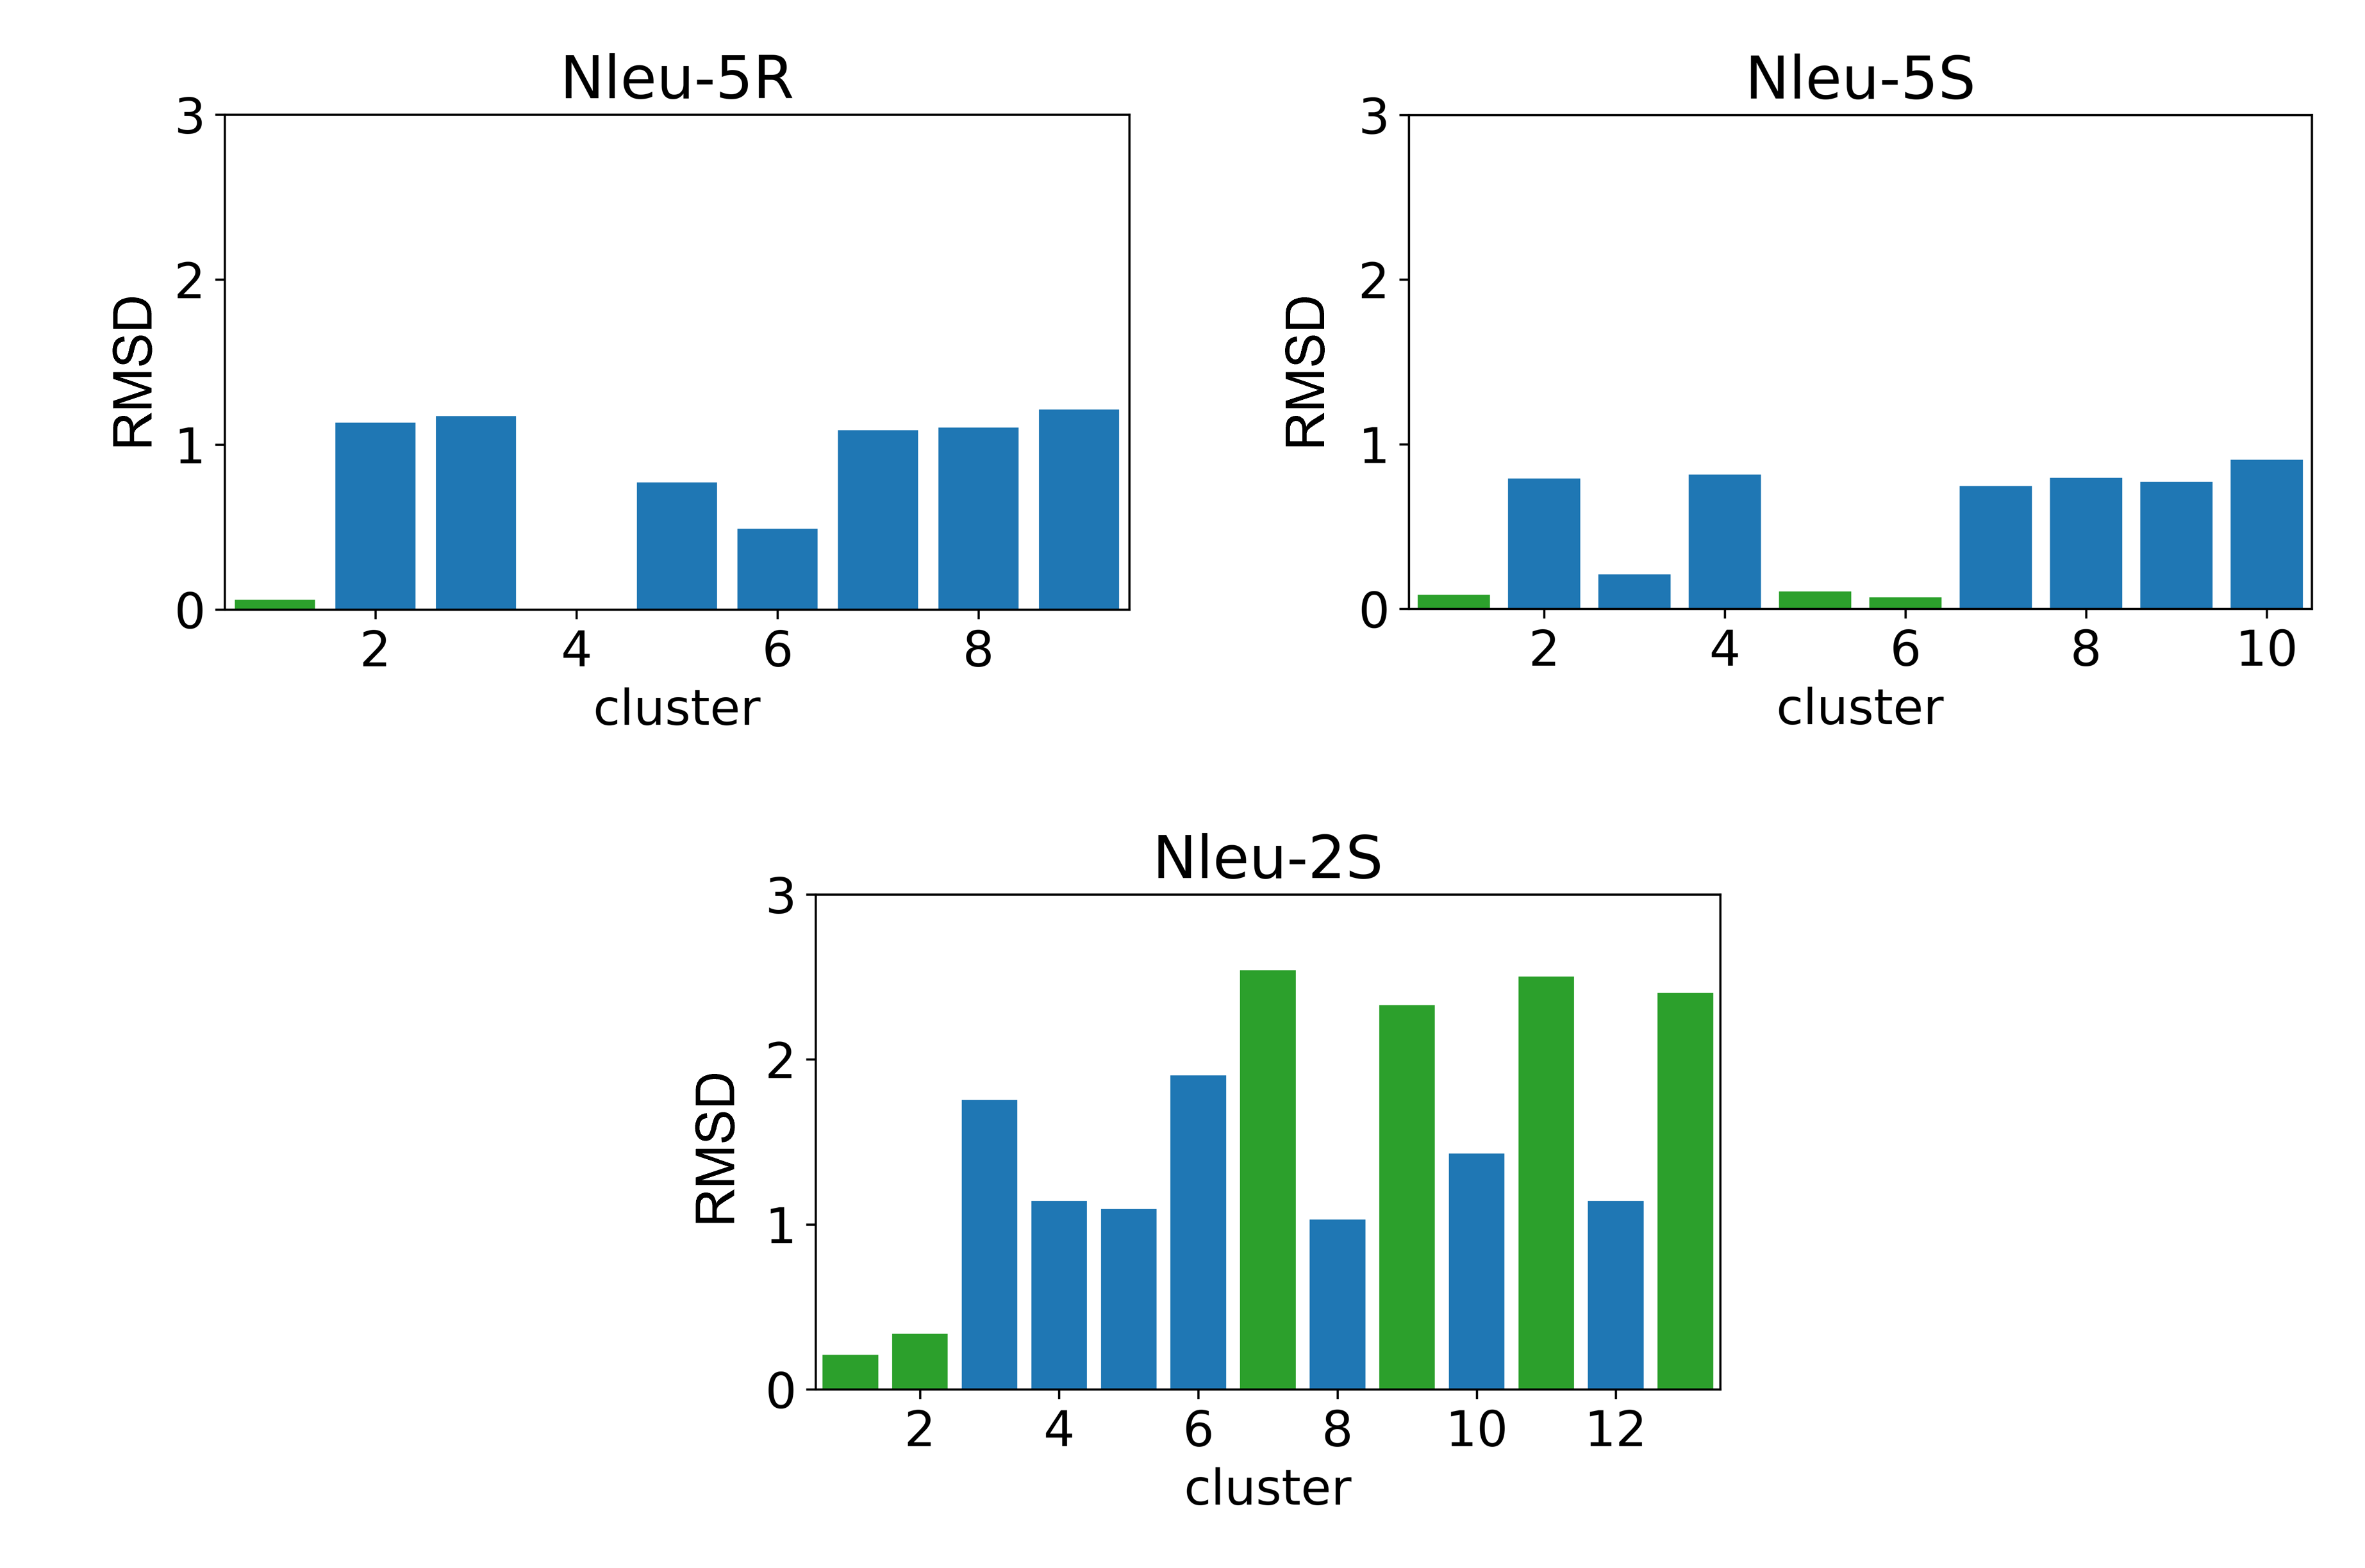
\includegraphics[width=\textwidth]{7_chapter_5/fig/results/j3NMRConfClusterAna.png}
    \caption{ Root-mean-square deviation (RMSD, in hertz) between $^3$J$_{\text{HN–H}\alpha}$ coupling constants in chloroform from NMR measurements and from MD simulations. Clusters with the peptoid bond in trans conformation are shown in green.}
    \label{fig: j3NMRConfClusterAna}
\end{figure}


The clusters with all amides in trans conformation are in good agreement with the  $^3J_{\text{HN–H}\alpha}$ coupling constants (Figure \ref{fig: j3NMRConfClusterAna}), whereas the clusters containing the cis-peptoid bond deviate significantly from the experimental values. For Nleu-2R, the $^3J_{\text{HN–H}\alpha}$ coupling analysis is missing as we could not determine the $^3J_{\text{HN–H}\alpha}$ couplings reliably due to line broadening in the spectrum. The NOE upper distance bounds are also generally reproduced in these clusters (Figures \ref{fig: SINOE violations Nleu-5S} -\ref{fig: SINOE violations Nleu-2SII}). Based on these findings, we focus the analysis in the following on those clusters, which have a reasonable agreement with the NMR data (i.e., clusters 1 and 4 for Nleu-5R, clusters 1, 5, and 6 for Nleu-5S, cluster 1 for Nleu-2R, and clusters 1 and 2 for Nleu-2S).

\begin{figure}[h!]
    \centering
    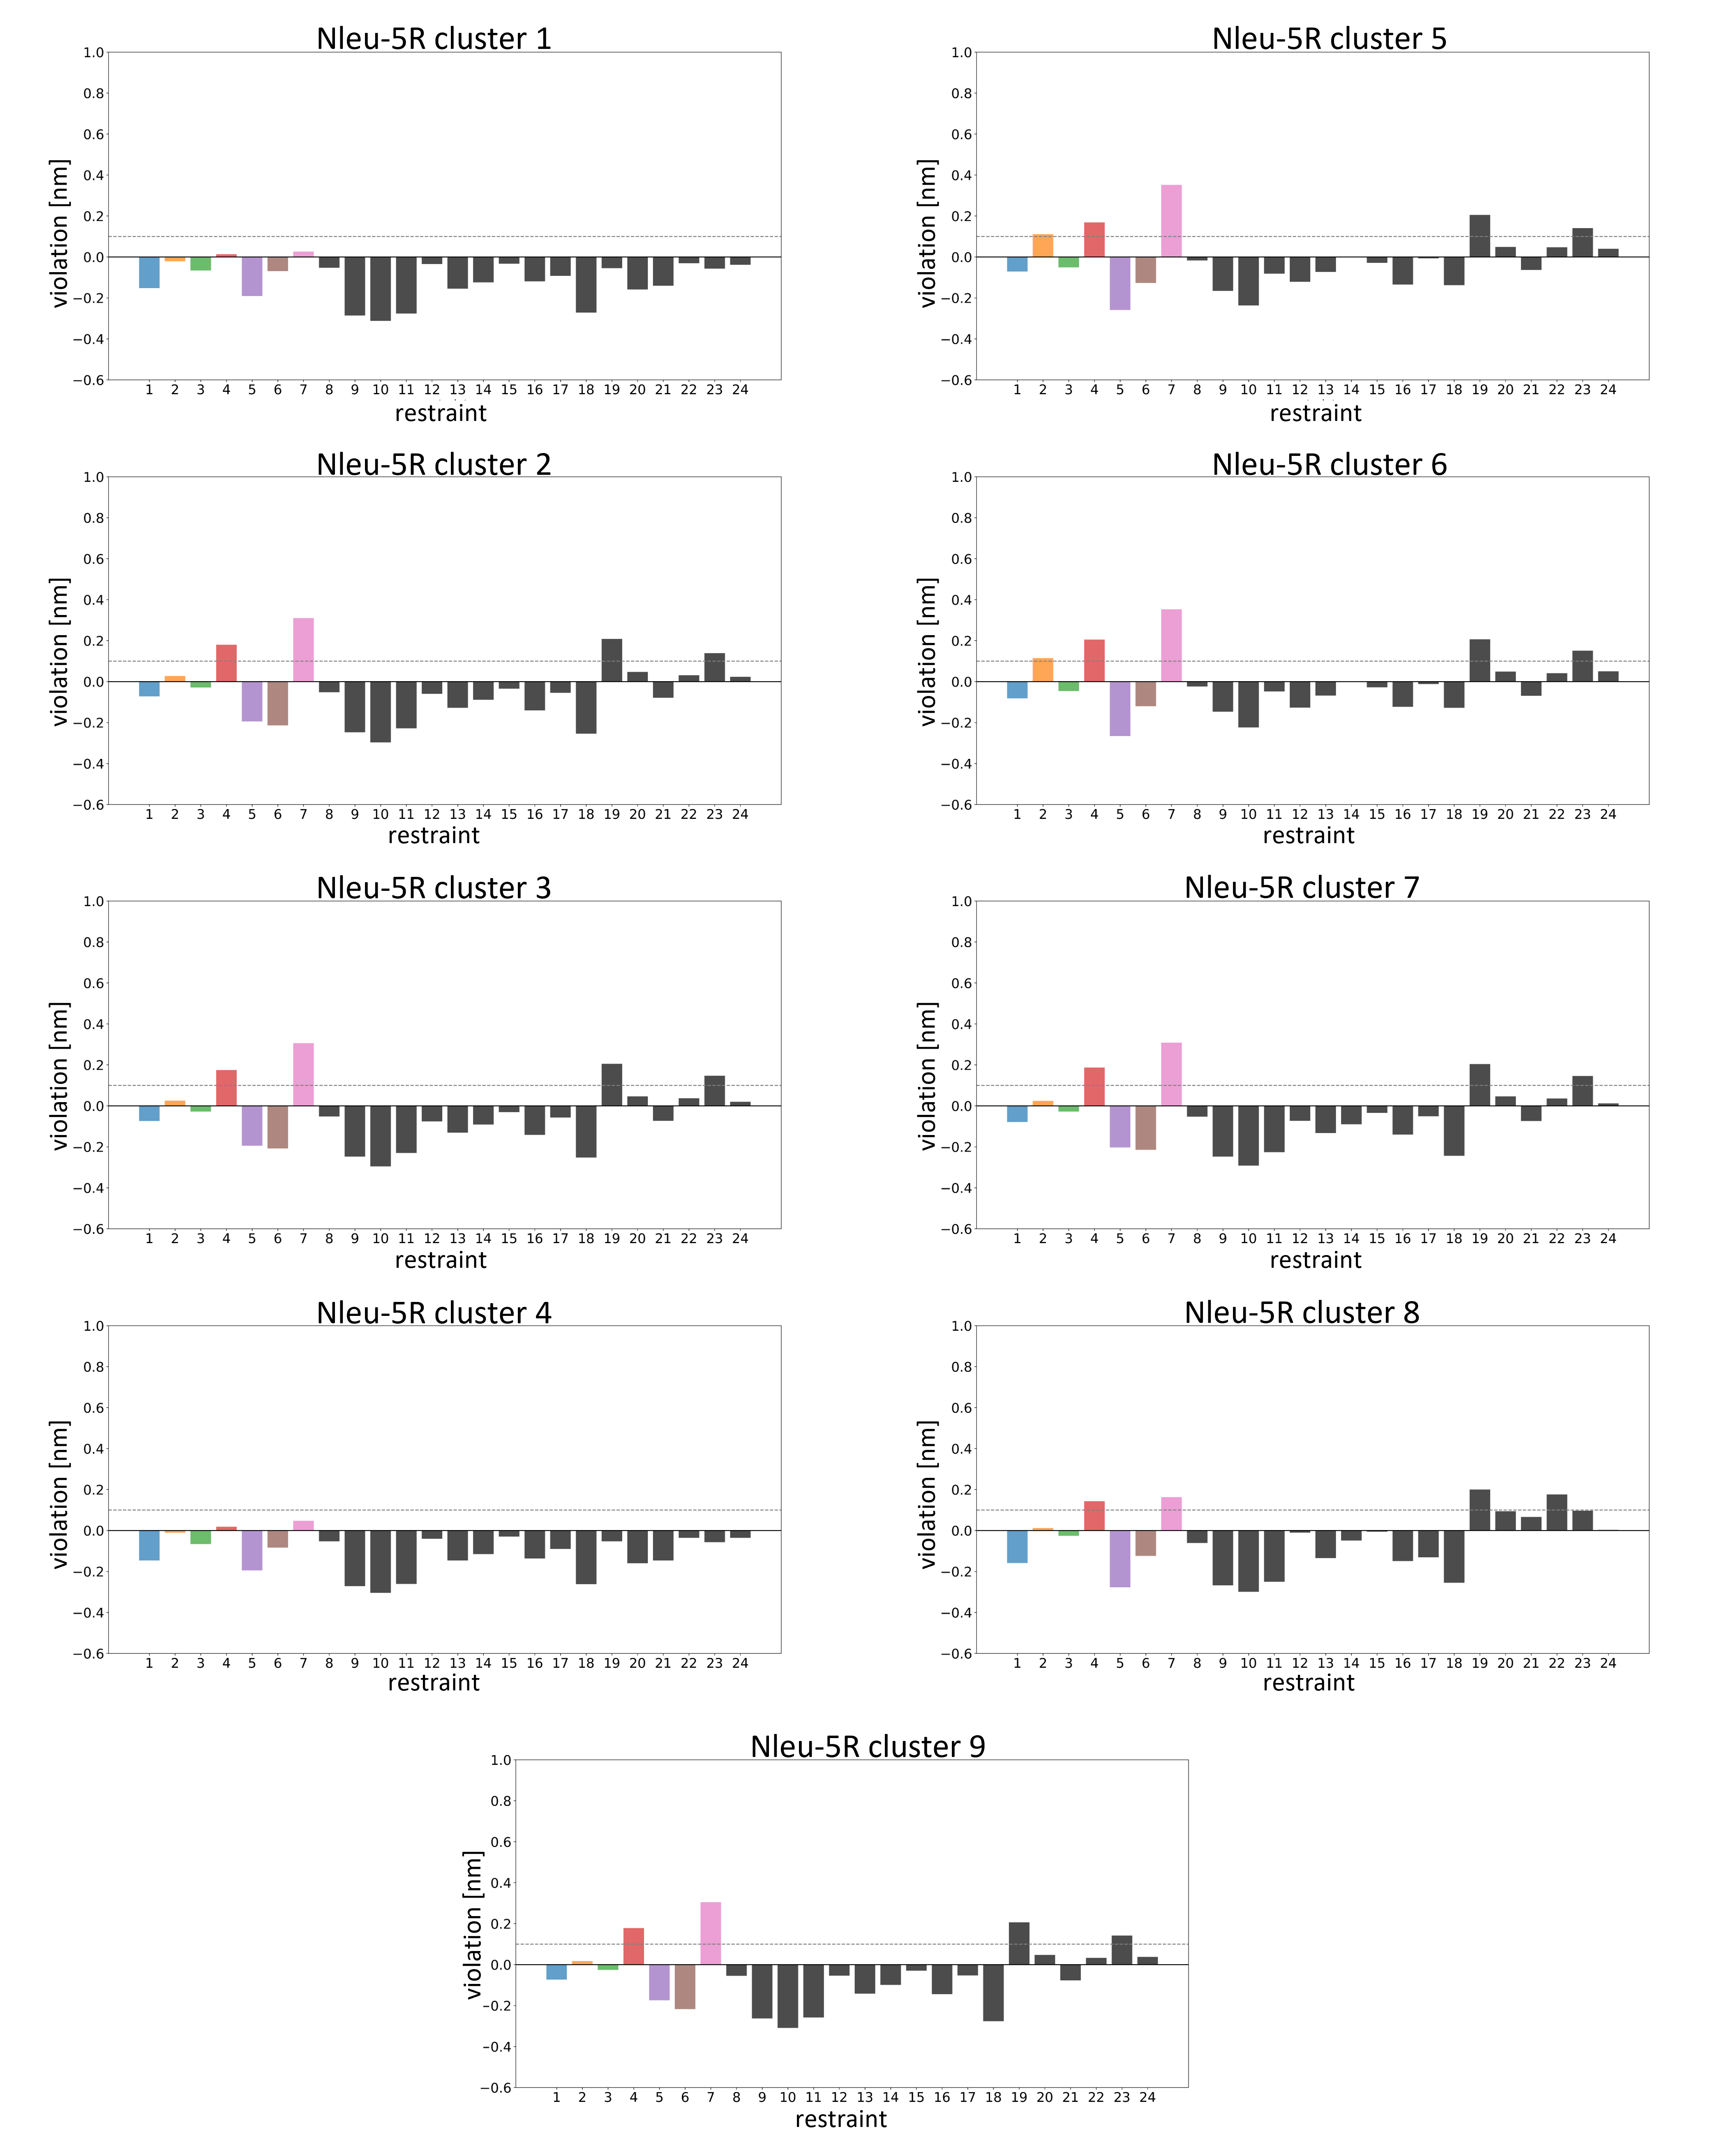
\includegraphics[width=\textwidth]{7_chapter_5/fig/results/NMR_5R.png}
    \caption{Violations  of  the  experimental  NOE  upper  distance  bounds  of  Nleu-5R  in chloroform by the clusters identified in the simulations in chloroform. Distances between residues across the backbone ring are colored. Distances between neighboring residues S22 are shown in black. The dashed line indicates the expected uncertainty of the NOE upper bounds.}
    \label{fig: SINOE violations Nleu-5R}
\end{figure}

\begin{figure}[h!]
    \centering
    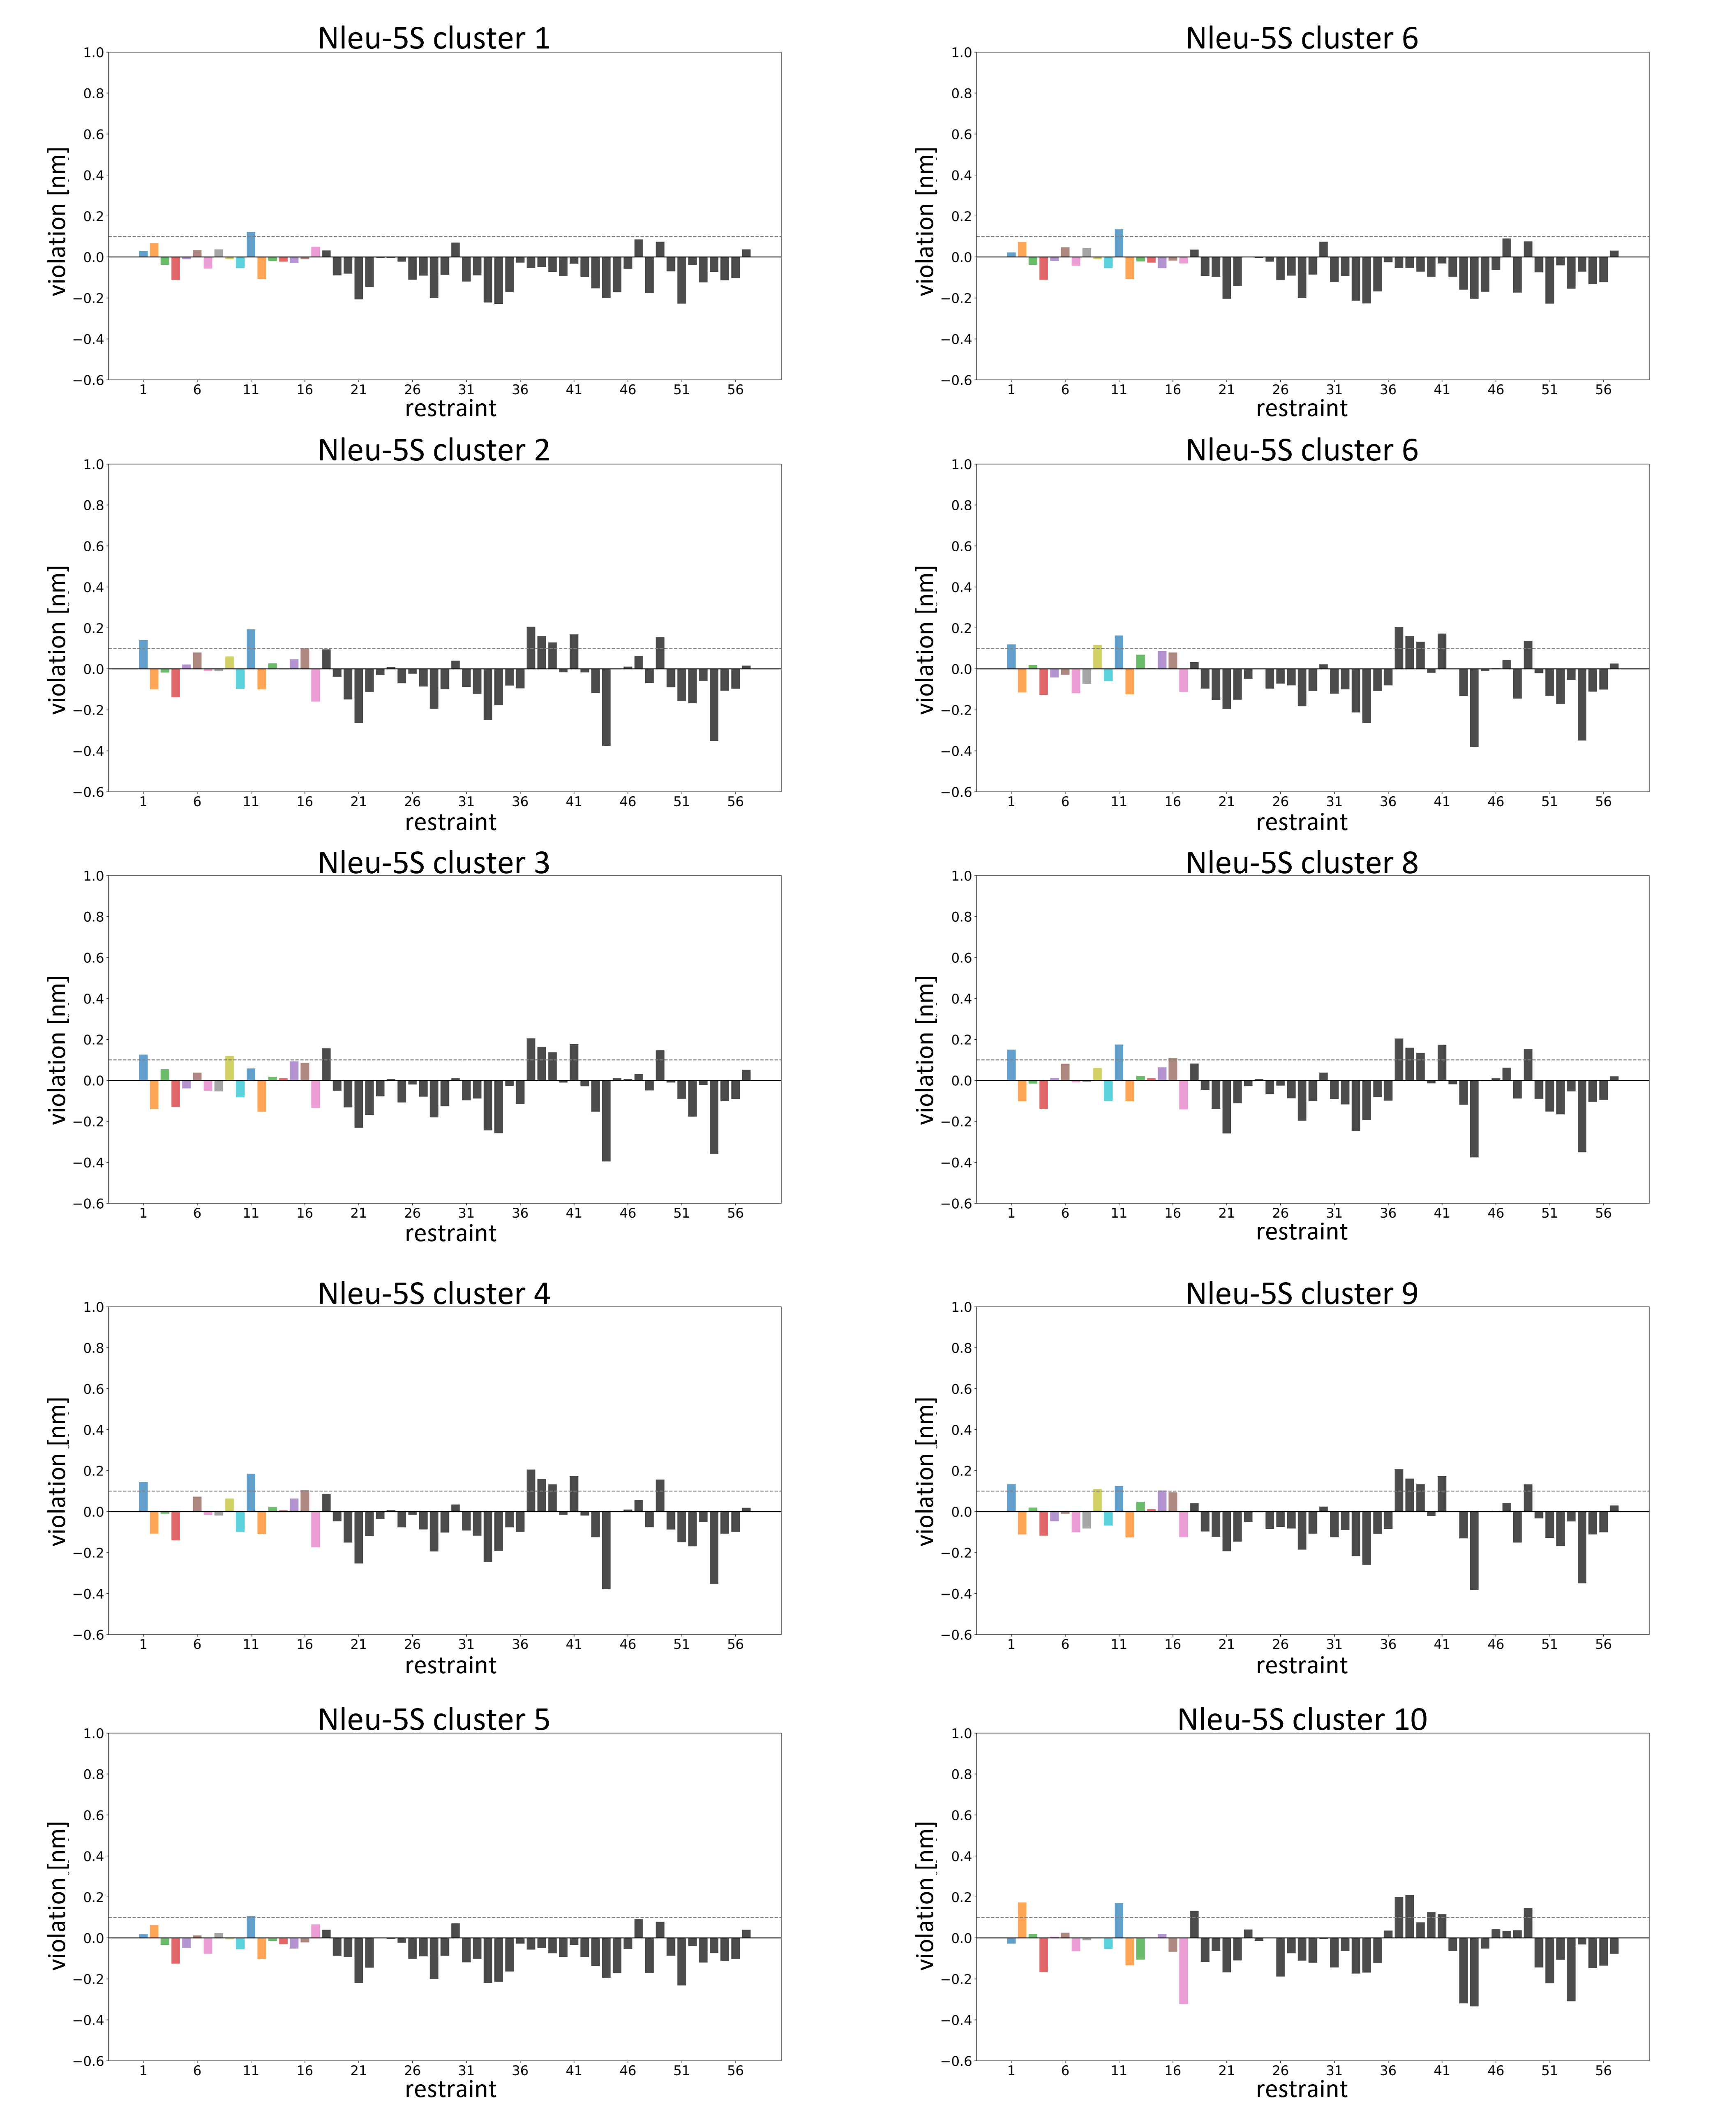
\includegraphics[width=\textwidth]{7_chapter_5/fig/results/NMR_5S.png}
    \caption{ Violations  of  the  experimental  NOE  upper  distance  bounds  of  Nleu-5S  in chloroform by the clusters identified in the simulations in chloroform. Distances between residues across the backbone ring are colored. Distances between neighboring residues are shown in black. The dashed line indicates the expected uncertainty of the NOE upper bounds.}
    \label{fig: SINOE violations Nleu-5S}
\end{figure}

\begin{figure}[h!]
    \centering
    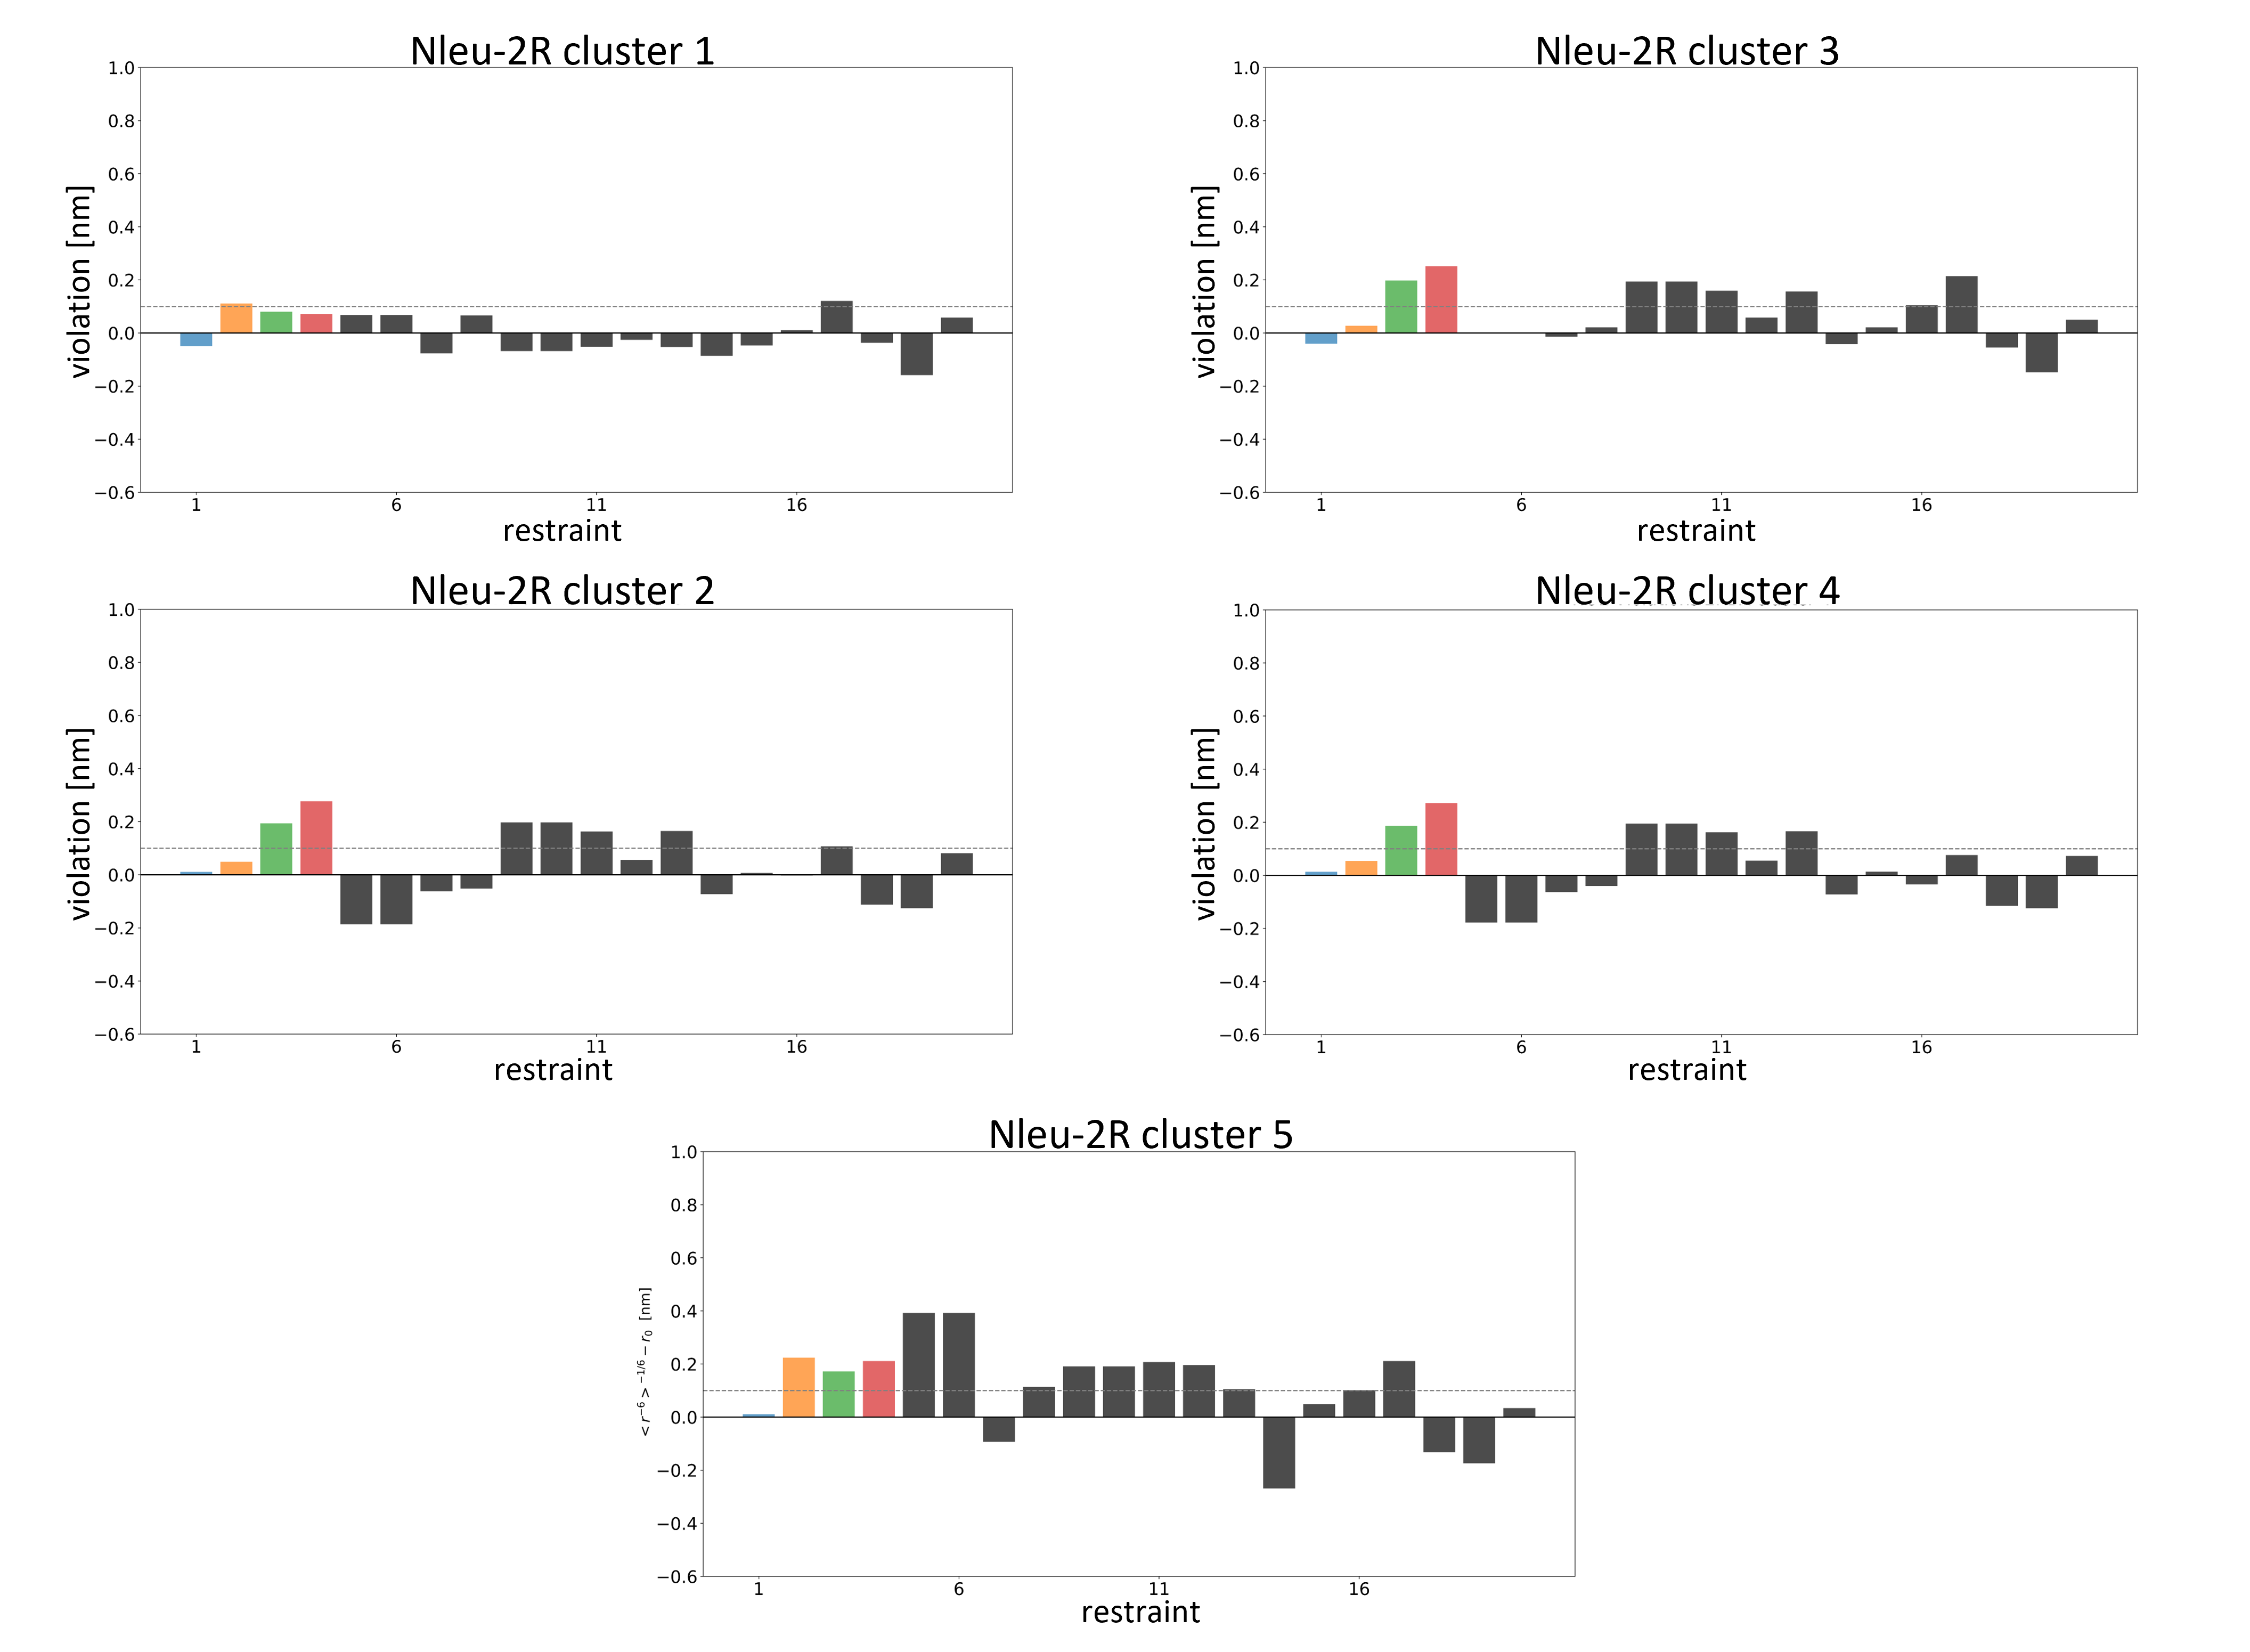
\includegraphics[width=\textwidth]{7_chapter_5/fig/results/NMR_2R.png}
    \caption{Violations  of  the  experimental  NOE  upper  distance  bounds  of  Nleu-2R  in chloroform by the clusters identified in the simulations in chloroform. Distances between residues across the backbone ring are colored. Distances between neighboring residues are shown in black. The dashed line indicates the expected uncertainty of the NOE upper bounds.}
    \label{fig: SINOE violations Nleu-2R}
\end{figure}

\begin{figure}[h!]
    \centering
    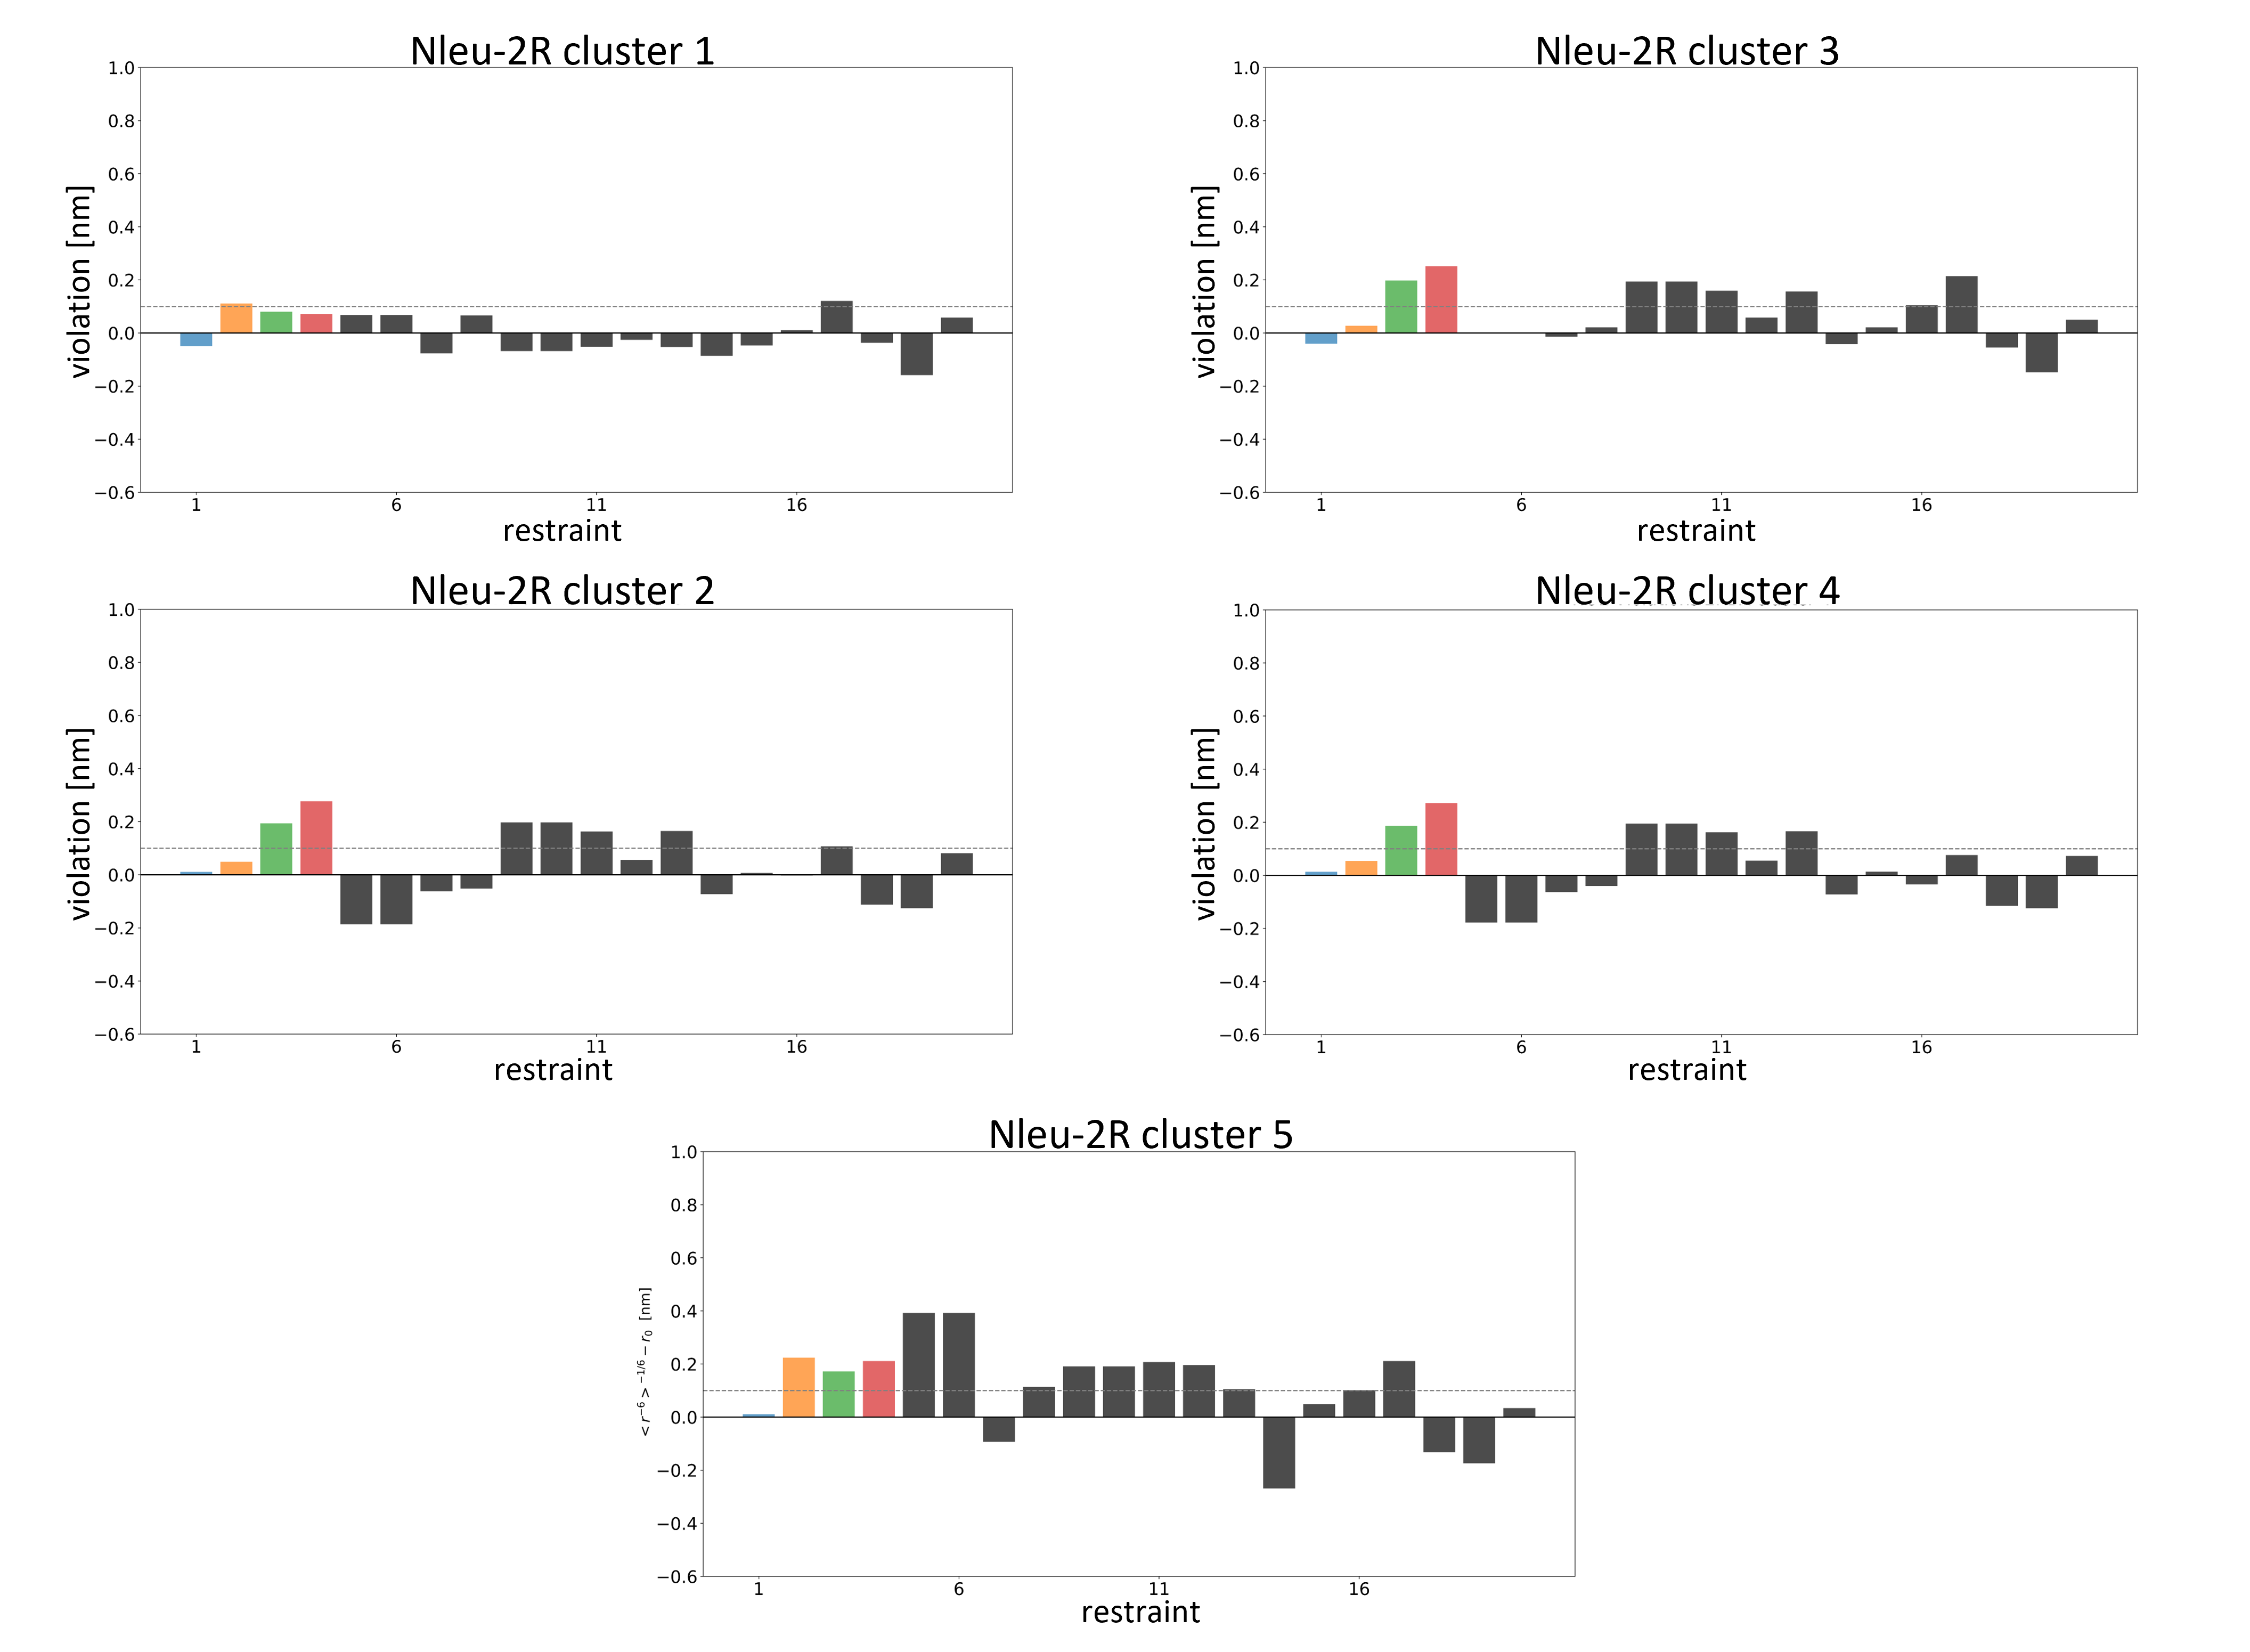
\includegraphics[width=\textwidth]{7_chapter_5/fig/results/NMR_2R.png}
    \caption{Violations  of  the  experimental  NOE  upper  distance  bounds  of  Nleu-2S  in chloroform by clusters 1–6 identified in the simulations in chloroform. Distances between residues across the backbone ring are colored. Distances between neighboring residues are shown in black. The dashed line indicates the expected uncertainty of the NOE upper bounds.}
    \label{fig: SINOE violations Nleu-2S}
\end{figure}

\begin{figure}[h!]
    \centering
    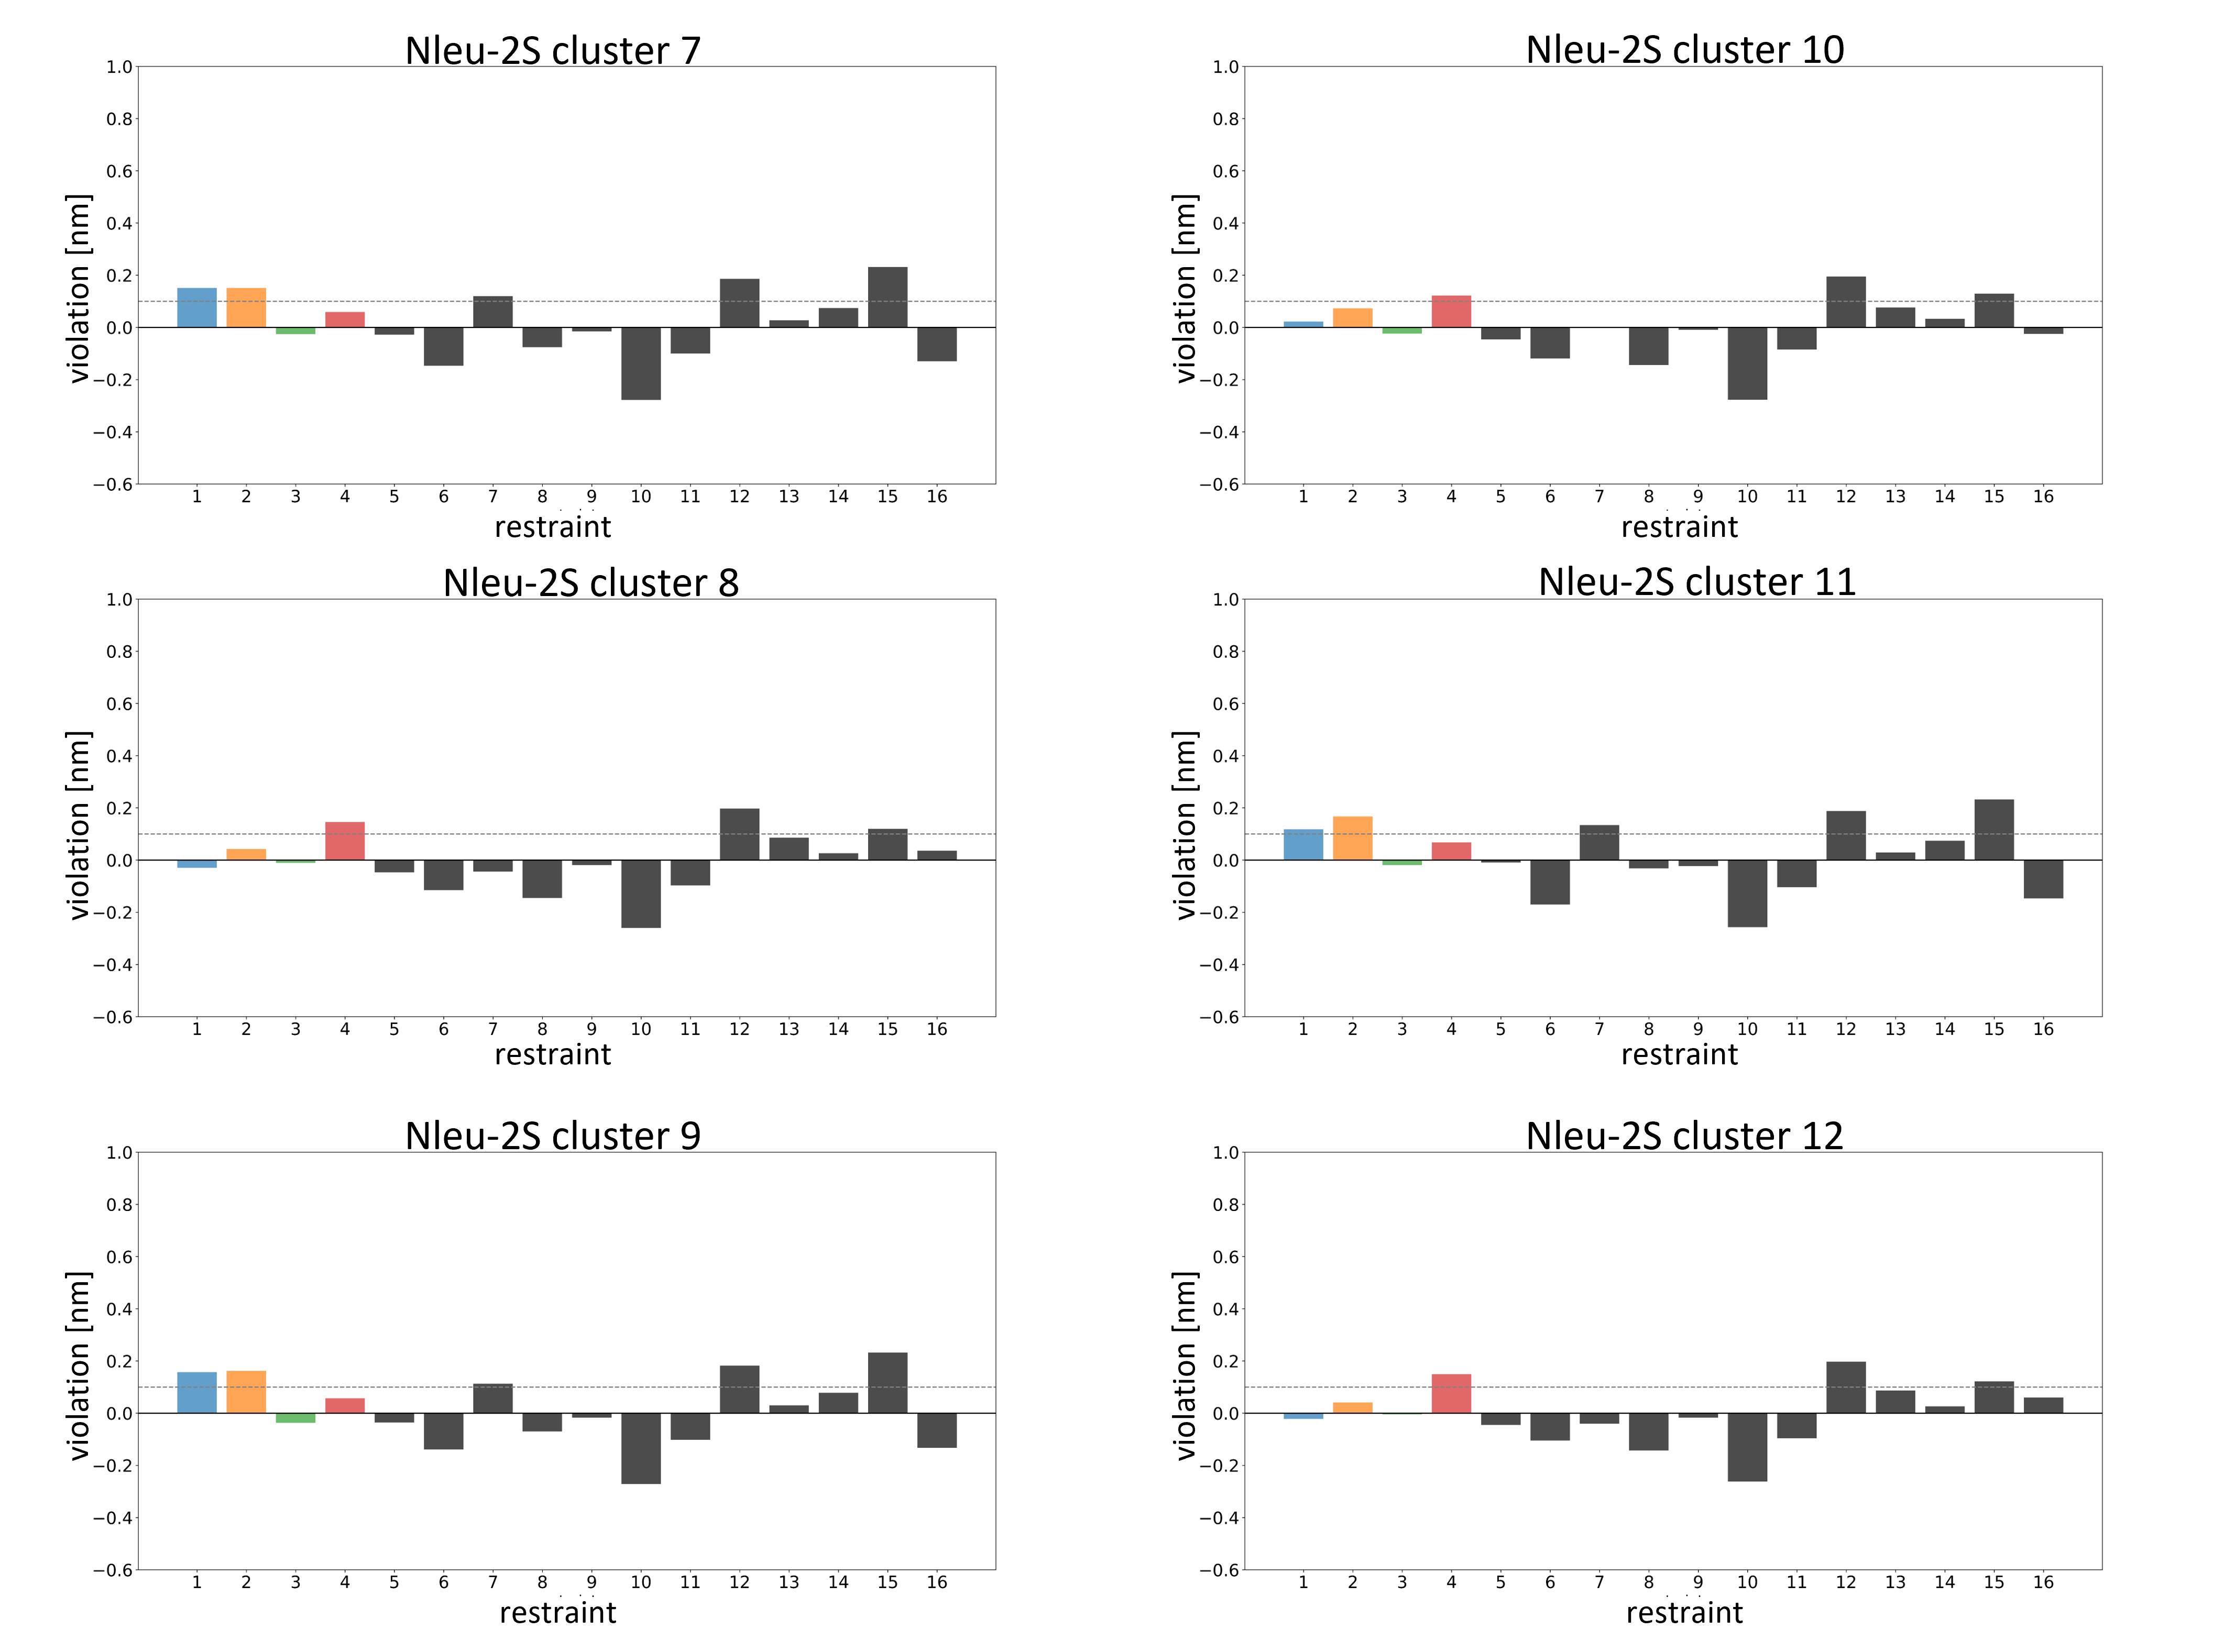
\includegraphics[width=\textwidth]{7_chapter_5/fig/results/NMR_2Sb.png}
    \caption{Violations  of  the  experimental  NOE  upper  distance  bounds  of  Nleu-2S  in chloroform by clusters 7–12 identified in the simulations in chloroform. Distances between residues across the backbone ring are colored. Distances between neighboring residues are shown in black. The dashed line indicates the expected uncertainty of the NOE upper bounds.}
    \label{fig: SINOE violations Nleu-2SII}
\end{figure}

\FloatBarrier
%-------------------------------------------

\subsection{Conformation Analysis}
A necessary condition for good membrane permeability is the adoption of conformations that shield polar groups optimally from the apolar environment. \cite{Sebastiano2018, Alex2011, Tyagi2018}
Therefore, we first analyzed the hydrogen-bonding patterns in the clusters in chloroform. For the peptides in this study, a maximum number of two H-bonds can be formed in a conformation due to ring strain. As can be seen in Table \ref{tab: hbondsratio}, the percentage of sampled conformations with two H-bonds differs significantly between Nleu-5R ($30\%$) and Nleu-5S ($7\%$). At the same time, the percentage of conformations without a H-bond is increased for Nleu-5S ($25\%$) compared to Nleu-5R ($8\%$). For the other pair, Nleu-2R and Nleu-2S, the percentages are more similar and in between those of Nleu-5R and Nleu-5S.


\begin{table}[h!]
    \centering
    \caption{Percentage of Sampled Conformations with Zero, One, or Two Hydrogen Bonds in Chloroform. Analysis was restricted to the clusters with the trans-peptoid bond.}
    \label{tab: hbondsratio}
    \begin{adjustbox}{max width=\textwidth}
    \begin{tabular}{lccc}
    number of hydrogen bonds [\%] &	0 &	1 &	2 \\
    \hline
    Nleu-5R  &	8	& 63	& 30 \\
    Nleu-5S  &	25	& 68	& 7  \\
    Nleu-2R  &	15	& 64	& 21 \\
    Nleu-2S  &	13	& 74	& 13 \\
    \hline
    \end{tabular}
    \end{adjustbox}
\end{table}

Analysis was restricted to the clusters with the trans-peptoid bond.
For a given molecule in an apolar environment, having access to conformations in which polar groups are shielded—such as by H-bonding—should be energetically favorable. 
To assess this effect, we extracted the potential energy of the peptides (i.e., intramolecular and peptide-solvent contributions) from the trajectories. 
The normality of each potential-energy distribution was confirmed by the Shapiro–Wilk test \cite{Shapiro1965} (Table \ref{tab: SIstatTestingNorm}). 

\begin{table}[h!]
\centering
\caption{ Average potential energy of the peptides  (i.e. sum of the intramolecular $\langle \text{V} \rangle$ contributions  and  the  peptide–solvent  contributions)  together  with  the  p-value  of  the Shapiro-Wilk test for the simulations in chloroform and water, respectively. The significance limit for the p-value was 0.05.}
\label{tab: SIstatTestingNorm}
\begin{adjustbox}{max width=\textwidth}
\begin{tabular}{r|cc|cc}
\multirow{2}{*}{Molecule} & \multicolumn{2}{l}{Chloroform} & \multicolumn{2}{l}{Water}        \\
    & $\langle \text{V} \rangle [\text{kJ}/\text{mol}]$ & $\text{p}_{\text{Shapiro-Wilk}}$ & $\langle \text{V} \rangle [\text{kJ}/\text{mol}]$ & $\text{p}_{\text{Shapiro-Wilk}}$  \\
    \hline
    Nleu-5R    & -217.08    & \~0.0          & -117.77  & \~0.0         \\
    Nleu-5S    & -208.39    &   $5.9*10^{-8}$  & -115.64  & $5.24*10^{-10}$ \\
    Nleu-2R    & -211.17    & \~0.0          & -117.84  & \~0.0         \\
    Nleu-2S    & -216.63    &   $7.6*10^{-39}$ & -116.91  & \~0.0   \\
    \hline
\end{tabular}%
\end{adjustbox}
\end{table}

\begin{table}[h!]
\centering
\caption{Results of the Fisher t-test to validate the significance of the deviations in the 
average potential energy of the peptides. The significance limit for the p-value was 0.05}
\label{tab: SIstatTestingDiff}
\begin{adjustbox}{max width=\textwidth}
\begin{tabular}{lcc}
Molecule          & Chloroform & Water     \\
\hline
Nleu-5R - Nleu-5S & $\sim$0.0  & $\sim$0.0 \\
Nleu-2R - Nleu-2S & $\sim$0.0  & $2.7*10^{-77}$\\
\hline
\end{tabular}%
\end{adjustbox}
\end{table}


The Fisher t-test \cite{Kotz1998} was employed to determine if the means of the distributions differ statistically significantly ($p < 0.05$). 
This was found to be the case for each pair of distributions (Table \ref{tab: SIstatTestingDiff}). 
On average, the potential energy of Nleu-5R is $9~$kJ/mol lower (i.e., more favorable) in chloroform compared to Nleu-5S, whereas the difference in the average potential energy between Nleu-2R and Nleu-2S is $6~$ kJ/mol. In many studies in the literature, it was found that the three-dimensional (3D) polar surface area (3D-PSA) is a good measure for the degree of polar shielding in conformations. \cite{Roux2020, Sebastiano2018, Vorherr2018, Peraro2018} 
However, for the present set of four peptides, no correlation was observed between the 3D-PSA and the potential energy (Figure \ref{fig: SI3DPSAANA}). 
\begin{figure}[h!]
    \centering
    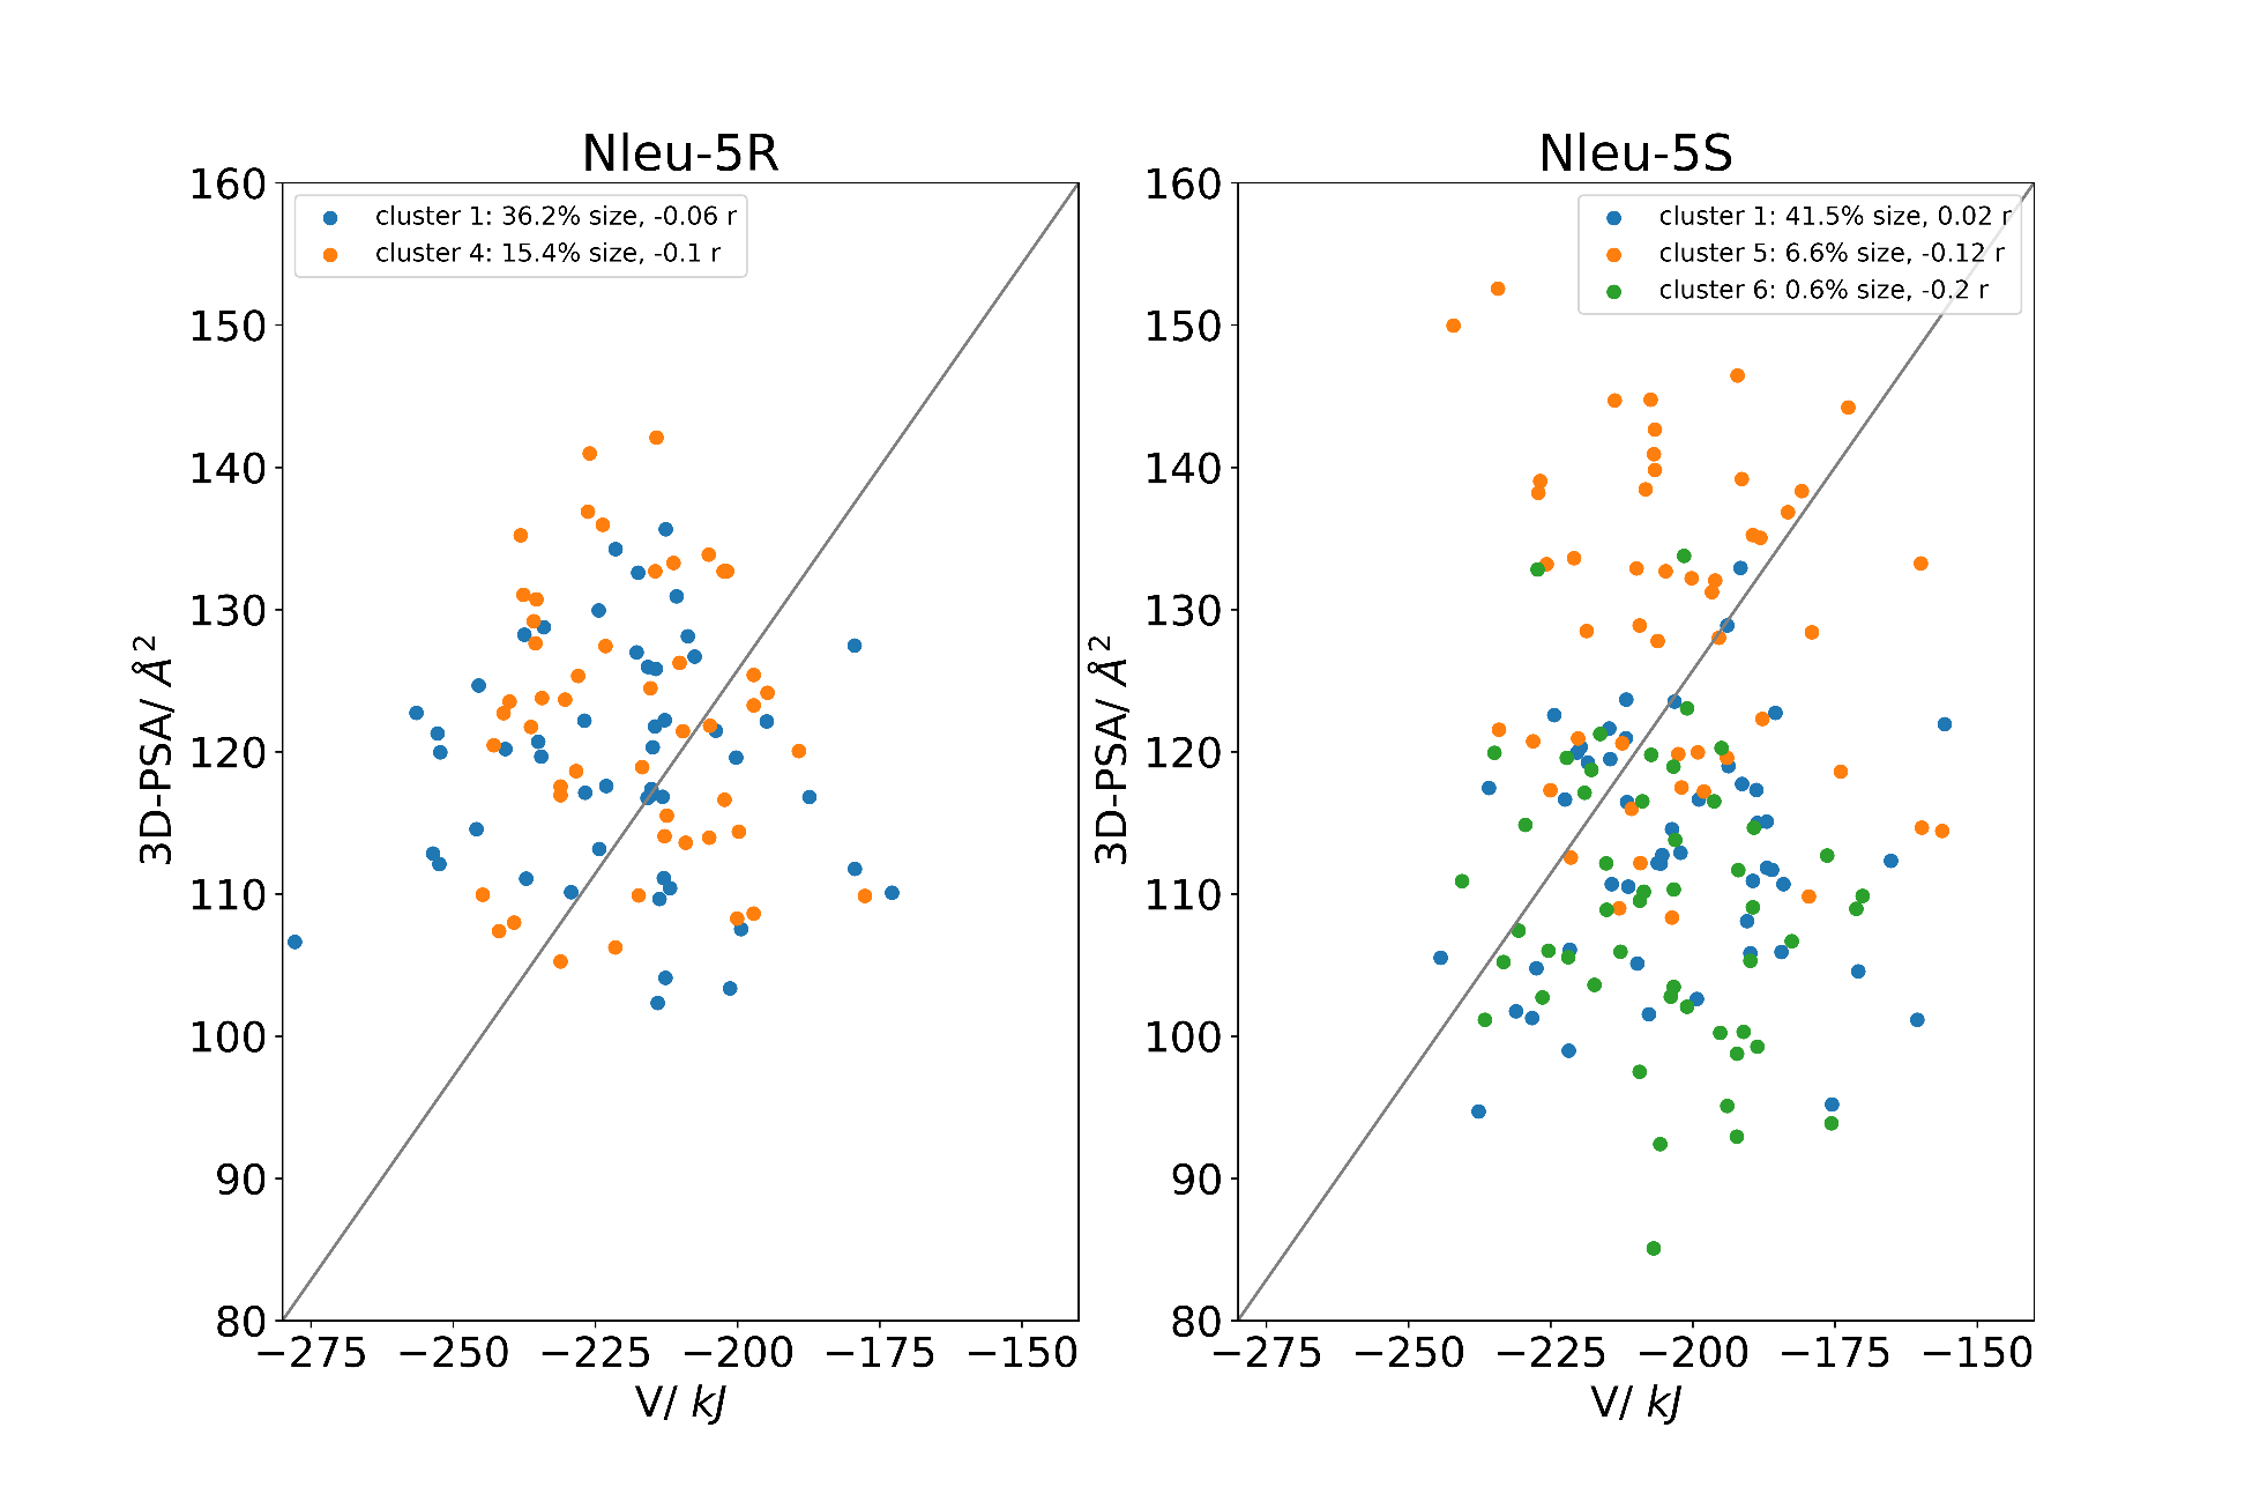
\includegraphics[width=\textwidth]{7_chapter_5/fig/results/3dPSA.png}
    \caption{Correlation between the 3D-PSA and the potential energy of the corresponding conformation (i.e. sum of intramolecular contributions and peptide–solvent 
        contributions) for Nleu-5R and Nleu-5S in chloroform. The 100 structures closest to the cluster  center  were  taken  for  the  clusters  with  the  trans-peptoid  bond.  The  trend  for  an expected  linear  correlation  is  shown  as  gray  line.  The  legend  contains  the  cluster population in percentage and the Spearman correlation coefficient r}
    \label{fig: SI3DPSAANA}
\end{figure}


The ring strain in the relatively small backbone cycle of the peptides affects the geometry of the intramolecular H-bonds, which is likely not reflected appropriately in the 3D-PSA calculation. 
In summary, the ranking Nleu-5R $<$ Nleu-2S $<$ Nleu-2R $<$ Nleu-5S, which was found in terms of both hydrogen-bonding patterns and potential energies, matches well with the experimental permeability data.
The findings described above indicate that the change in stereochemistry of the methyl group in position $5$ between Nleu-5R and Nleu-5S leads to different conformational behavior. 
A detailed analysis of the H-bonds showed that only Nleu-5S forms a H-bond between Ala-O and the tether-NH with an occurrence of $24\%$ in chloroform (Table 3). 
This H-bond across the ring of Nleu-5S prevents the formation of other H-bonds (Figure \ref{fig: HbondExamples}B).
Such a conformation with a single H-bond is likely less favorable (compared to one with more H-bonds) in chloroform because less polar groups are shielded. In the dominant conformation of Nleu-5R, on the other hand, two H-bonds can be formed across the ring (Figure \ref{fig: HbondExamples}A).
\begin{figure}[h!]
    \centering
    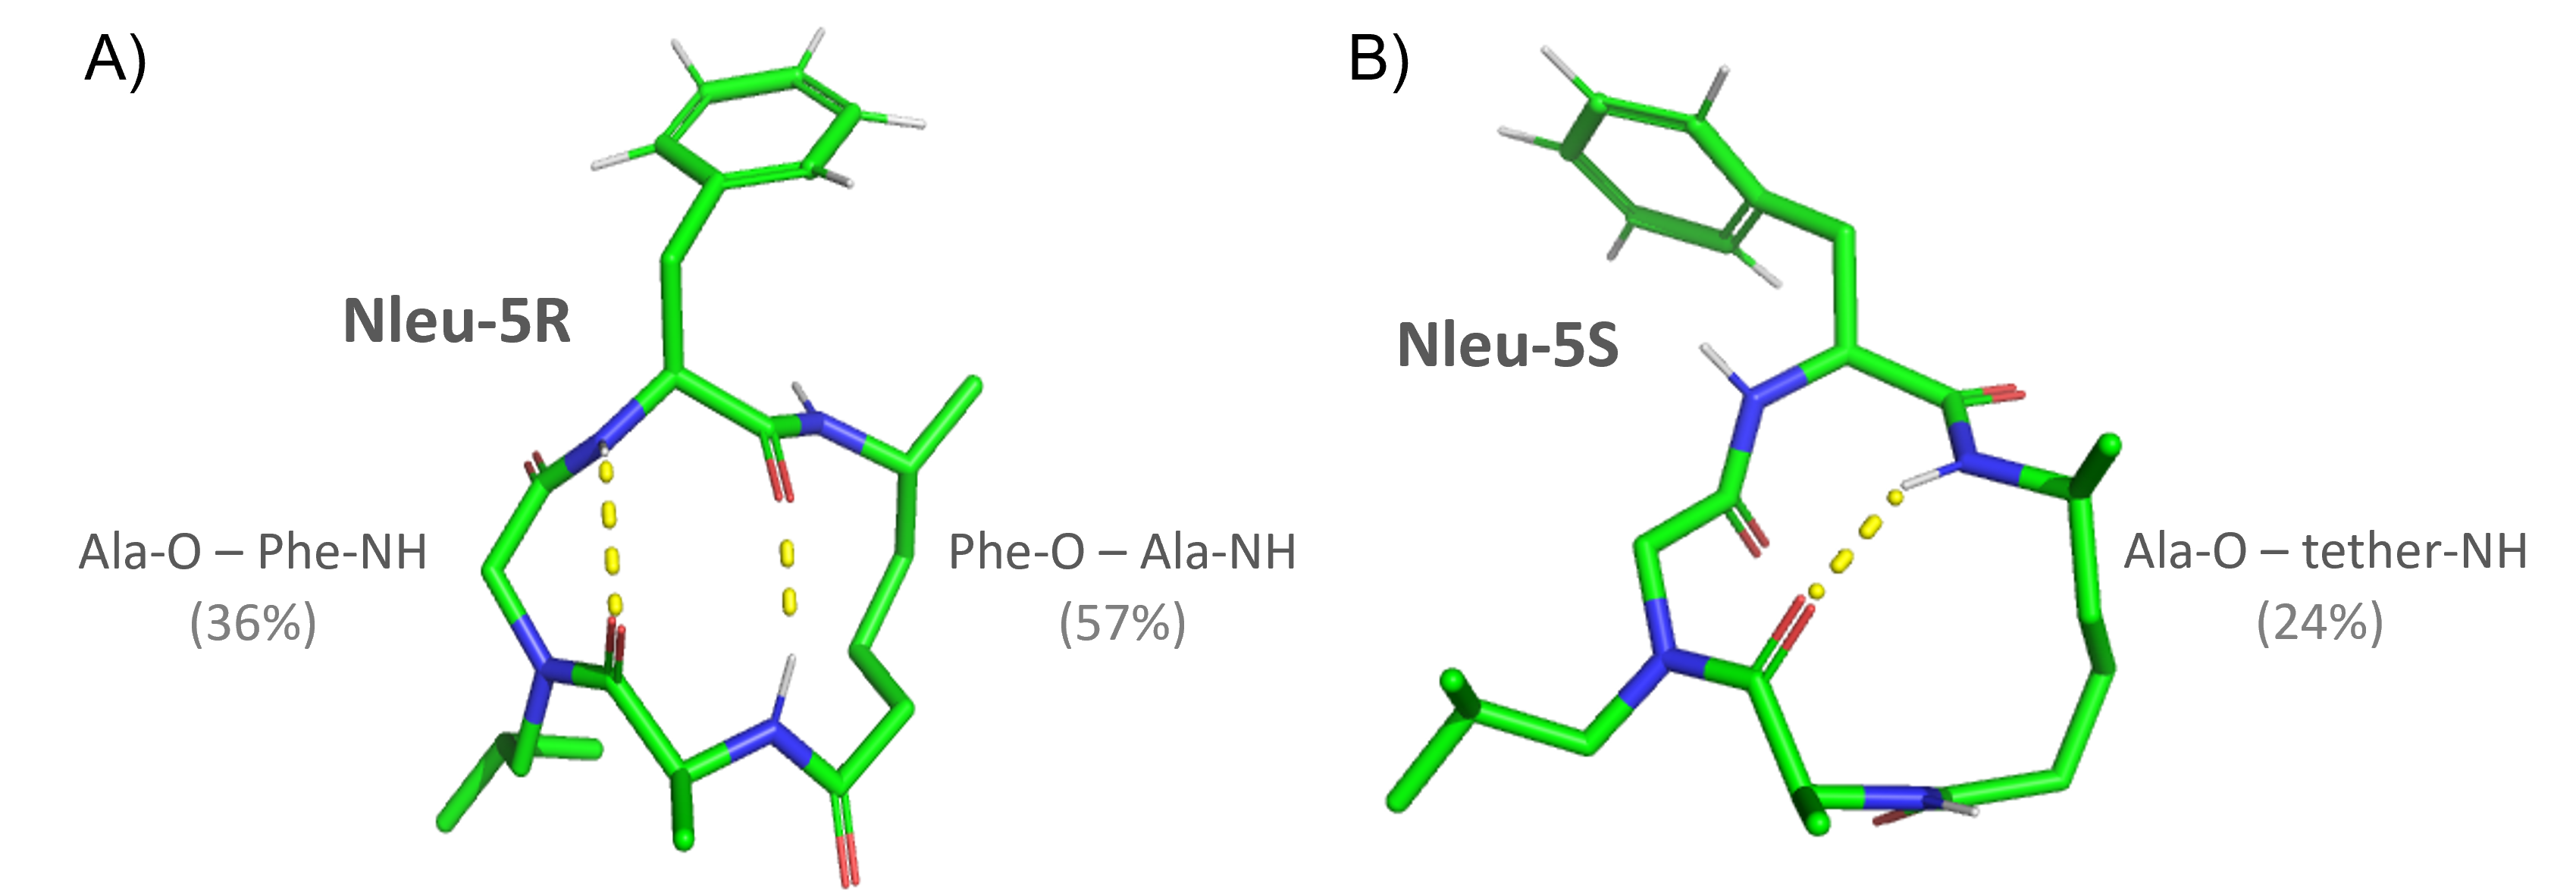
\includegraphics[width=\textwidth]{fig/results/ExampleHbonds.png}
    \caption{Snapshots of Nleu-5R (A) and Nleu-5S (B) from MD simulations in chloroform. Hydrogen bonds are shown with their percentage of the absolute occurrence in chloroform in the trans-peptoid clusters. Pictures were generated with PyMol. \cite{Delano2020}}
    \label{fig: HbondExamples}
\end{figure}

\begin{table}[h!]
    \centering
    \caption{Hydrogen Bond Occurrence in Percentage for the Sampled Conformations in Chloroform. Analysis was restricted to the clusters with the trans-peptoid bond.}
    \label{tab: hbondsrationCLCH3}
    \begin{adjustbox}{max width=\textwidth}
    \begin{tabular}{lcccc}
    H-bond  [\%] &	Nleu-2R &	Nleu-2S &	Nleu-5R &	Nleu-5S  \\
    \hline
    Nleu-O tether-NH &	74 &	37 &	28 &	33 \\
    Ala-O tether-NH &	\textless{}1 & \textless{}1 &	\textless{}1 &	24 \\
    Phe-O Ala-NH    &	\textless{}1 &	35 &	57 &	\textless{}1 \\
    Ala-O Phe-NH    &	27 &	25 &	36 &	17 \\
    \hline\\
    \end{tabular}
    \end{adjustbox}
\end{table}

Analysis was restricted to the clusters with the trans-peptoid bond.
Next, we analyzed the torsional-angle distributions in the backbone ring of the peptides. The change in stereochemistry of the methyl group at position 5 leads to a shift in the torsional-angle distributions of the tether units for Nleu-5S compared to Nleu-5R (Figure \ref{fig: dihedralDist}A). This shift results in a bent conformation of the ring (Figure 9B), which allows only one H-bond to form between Ala-O and tether-NH (Figure \ref{fig: dihedralDistSubst}). There is also a shift in the backbone torsional-angle distributions between Nleu-2R and Nleu-2S, however, to a much smaller extent (Figure \ref{fig: SITorsion2RS}).

\begin{figure}[h!]
    \centering
    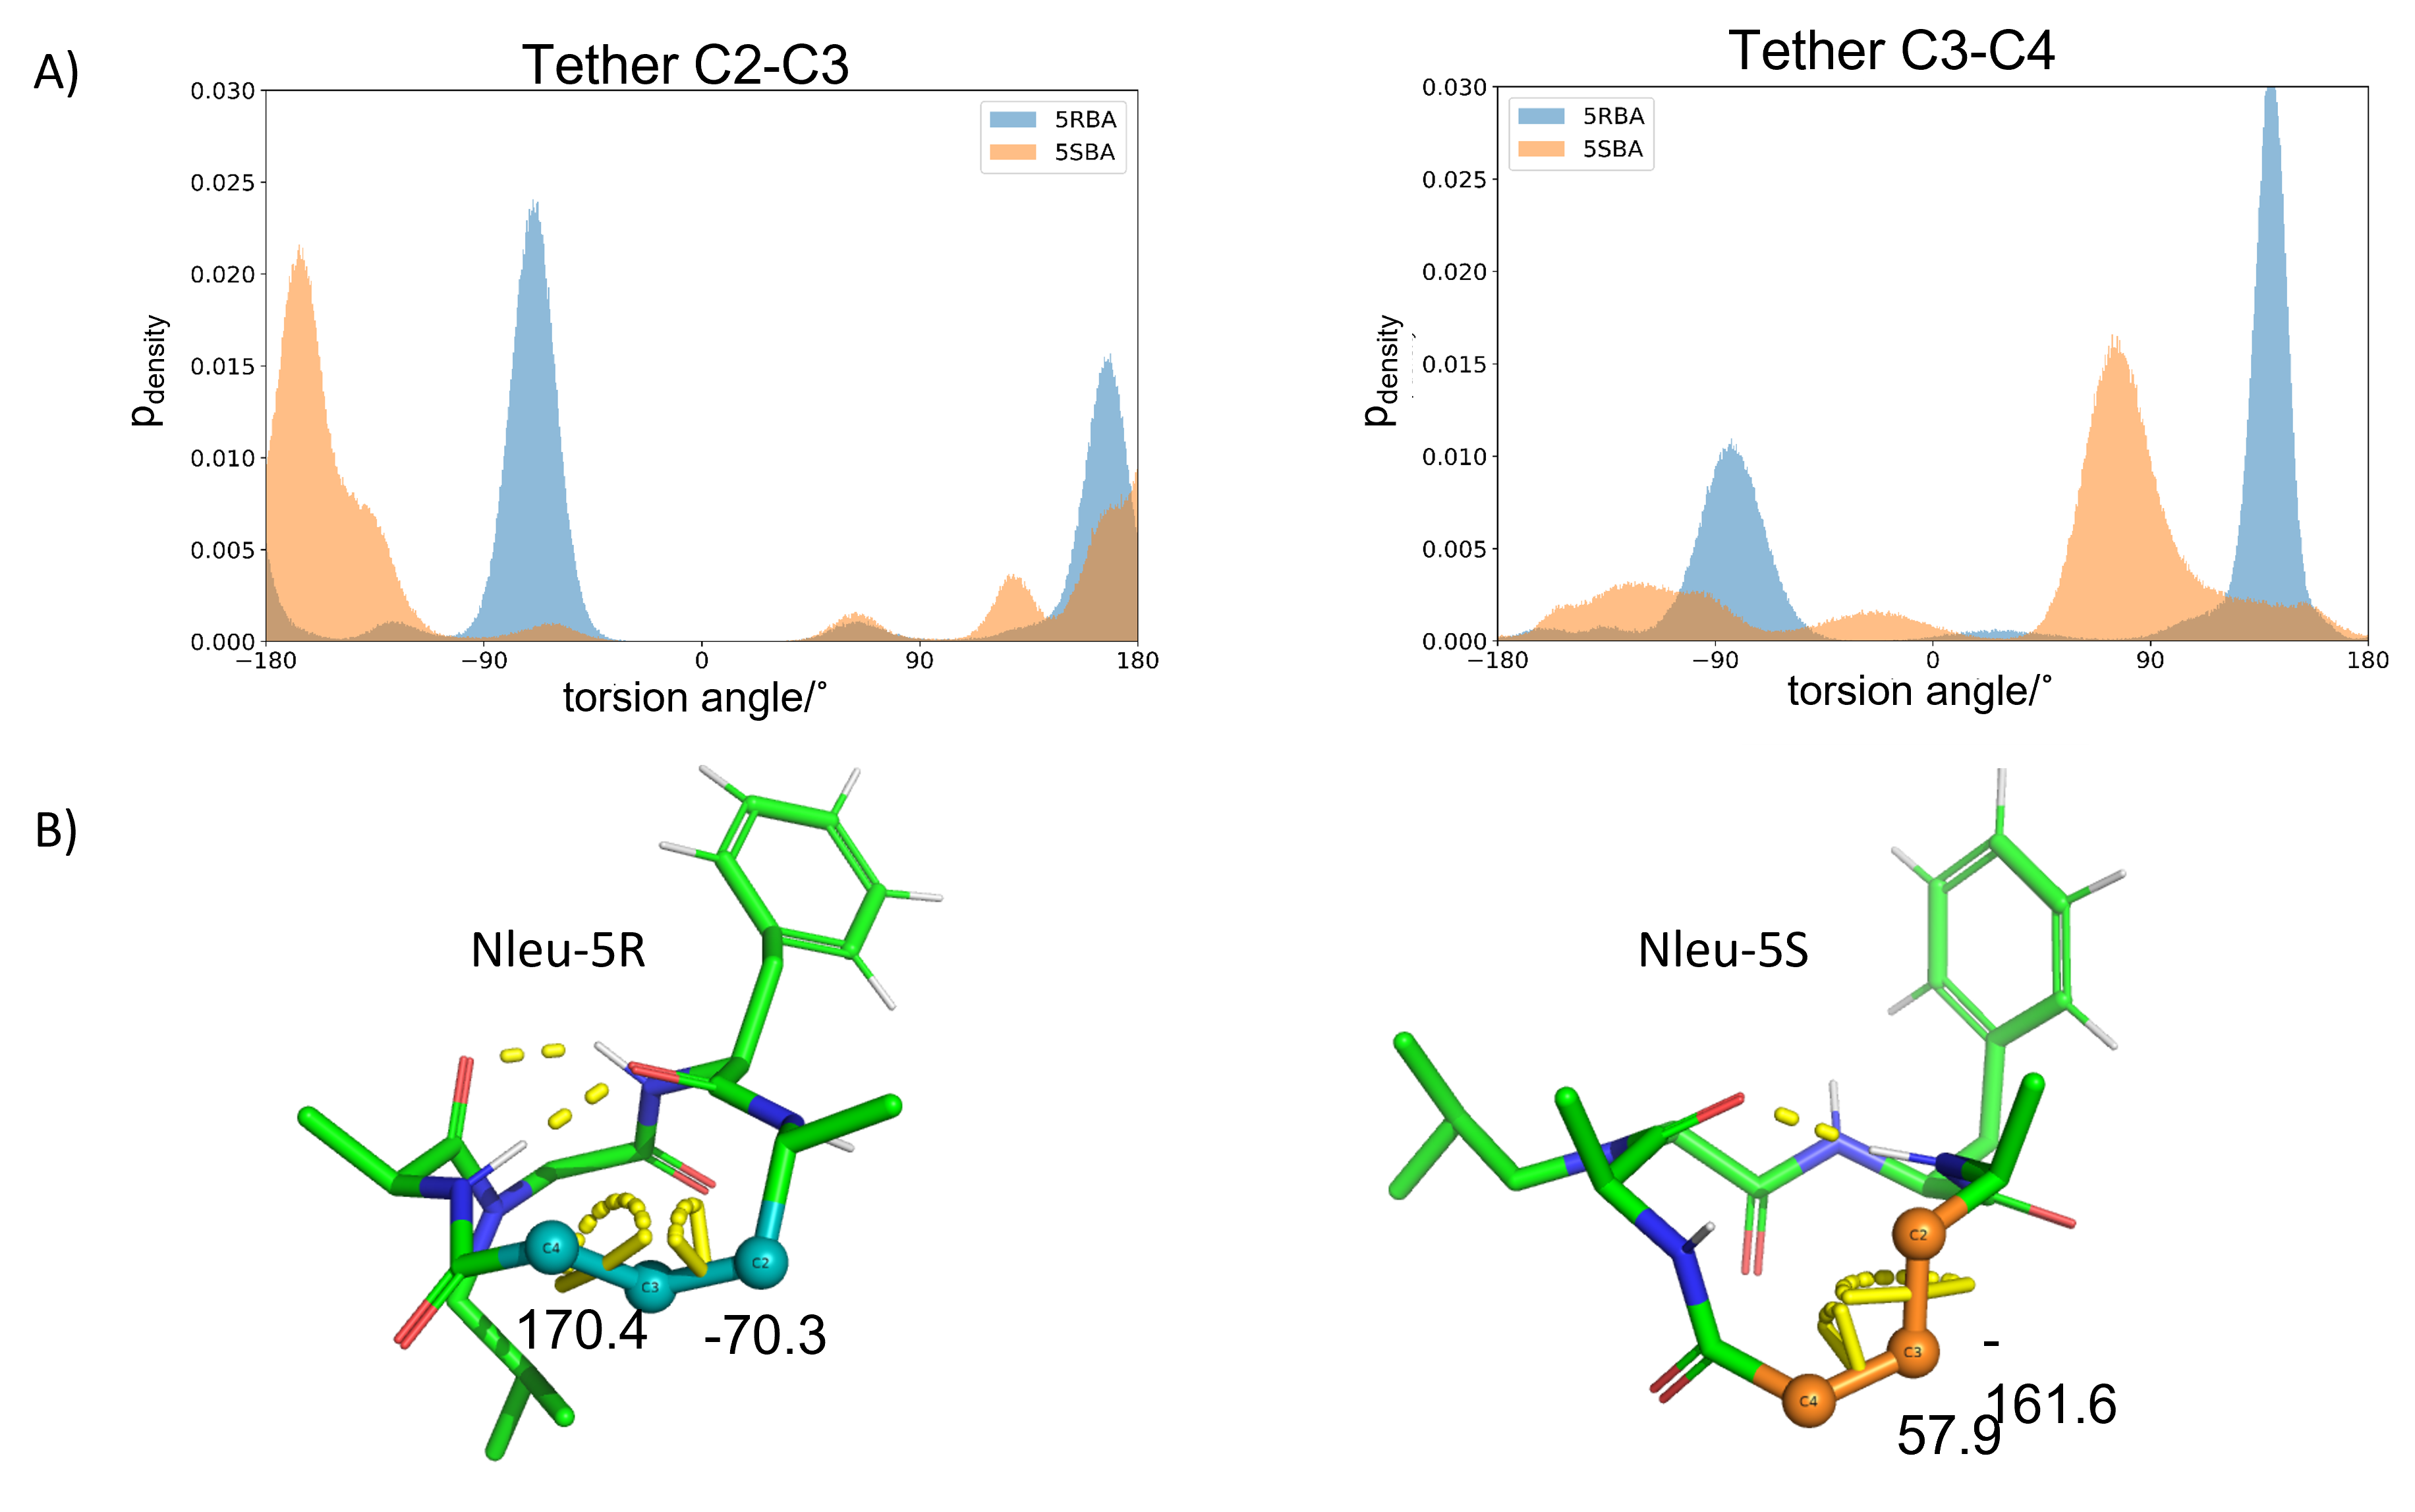
\includegraphics[width=\textwidth]{7_chapter_5/fig/results/dihedral_dist.png}
    \caption{(A) Torsional-angle distributions of the tether in Nleu-5R (blue) and Nleu-5S (orange) in chloroform. The analysis was restricted to the clusters with the trans-peptoid bond. (B) Torsional angles of the tether (shown in cyan and orange) corresponding to the peaks of the distributions. Pictures were generated with PyMol. \cite{Delano2020} The change in the stereocenter also affects the χ1-angle of the phenylalanine residue as the tether conformation hinders the rotation around this torsion due to a steric clash with the carbonyl group that is facing out of the backbone ring (Figure \ref{fig: dihedralDistSubst}).
    }
    \label{fig: dihedralDist}
\end{figure}

\begin{figure}[h!]
    \centering
    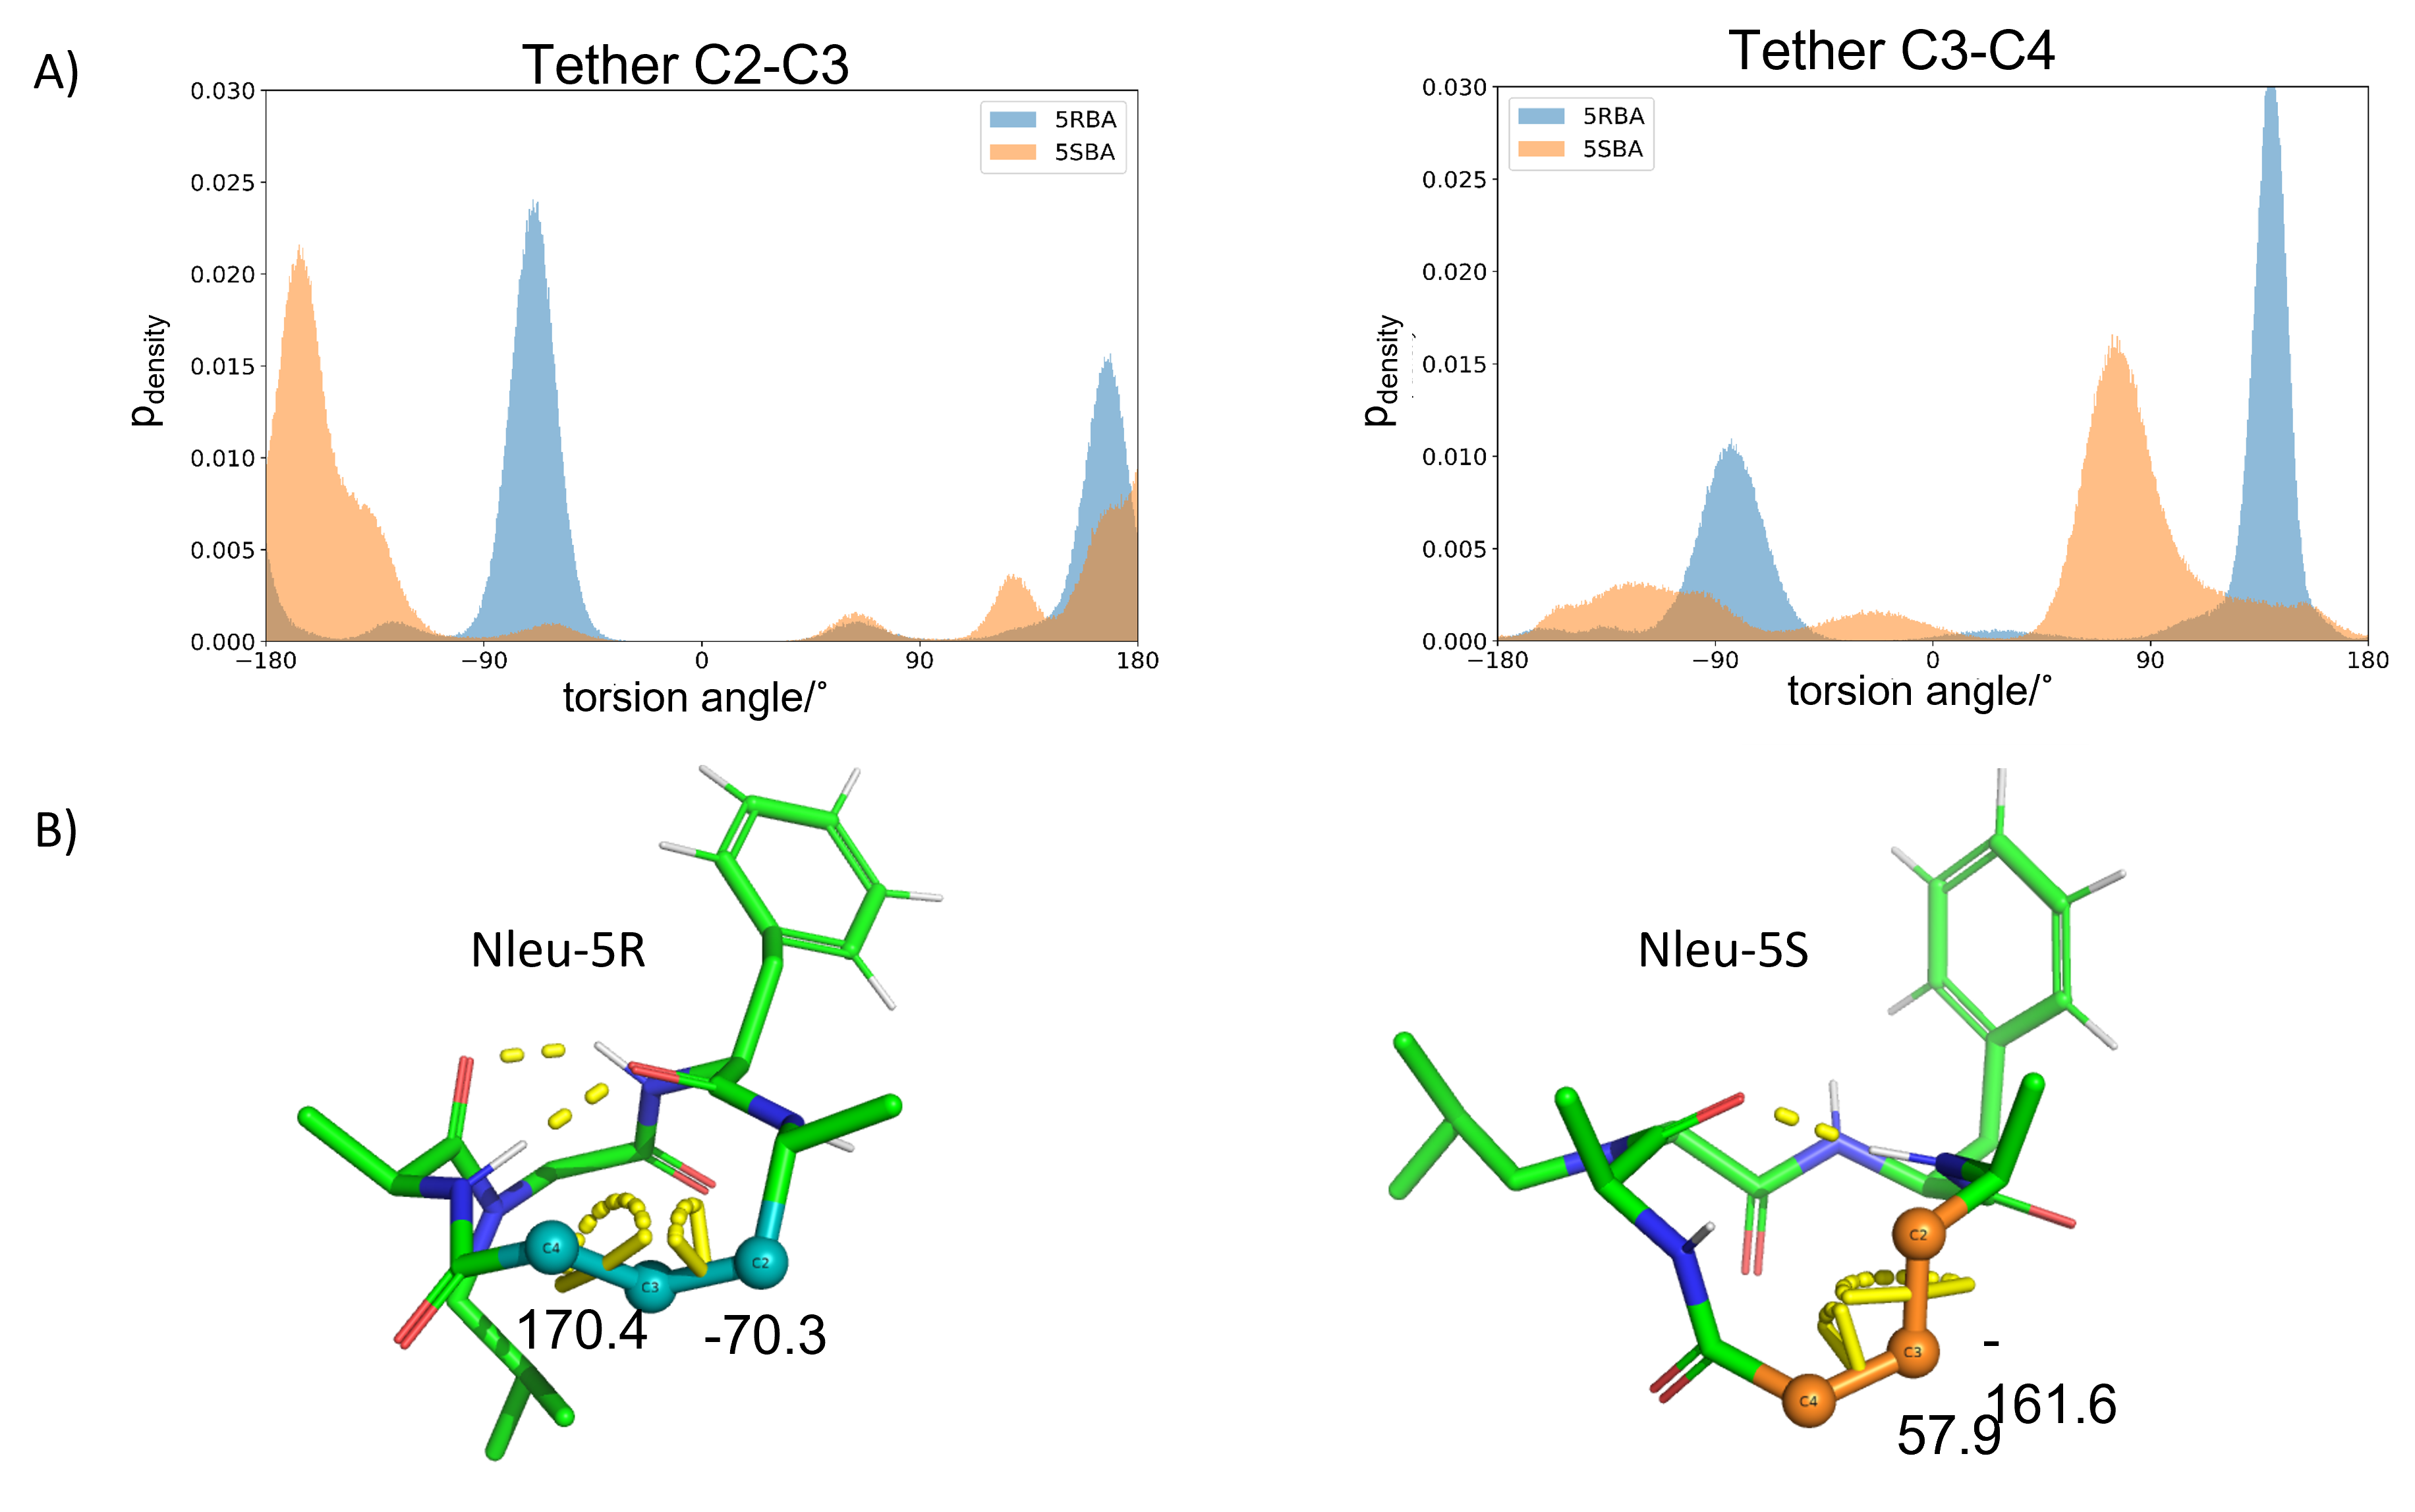
\includegraphics[width=\textwidth]{7_chapter_5/fig/results/dihedral_dist.png}
    \caption{(A) Torsional-angle distributions of the χ1 torsional angle of the phenylalanine residue in Nleu-5R (blue) and Nleu-5S (orange) in chloroform. Analysis was restricted to the clusters with the trans-peptoid bond. (B) χ1 torsional angle of the phenylalanine residue (shown in purple) corresponding to the peaks of the distributions. The backbone carbonyl interferes with the rotation around this torsion is highlighted with a red circle. Pictures were generated with PyMol. \cite{Delano2020}}
    \label{fig: dihedralDistSubst}
\end{figure}

\begin{figure}[h!]
    \centering
    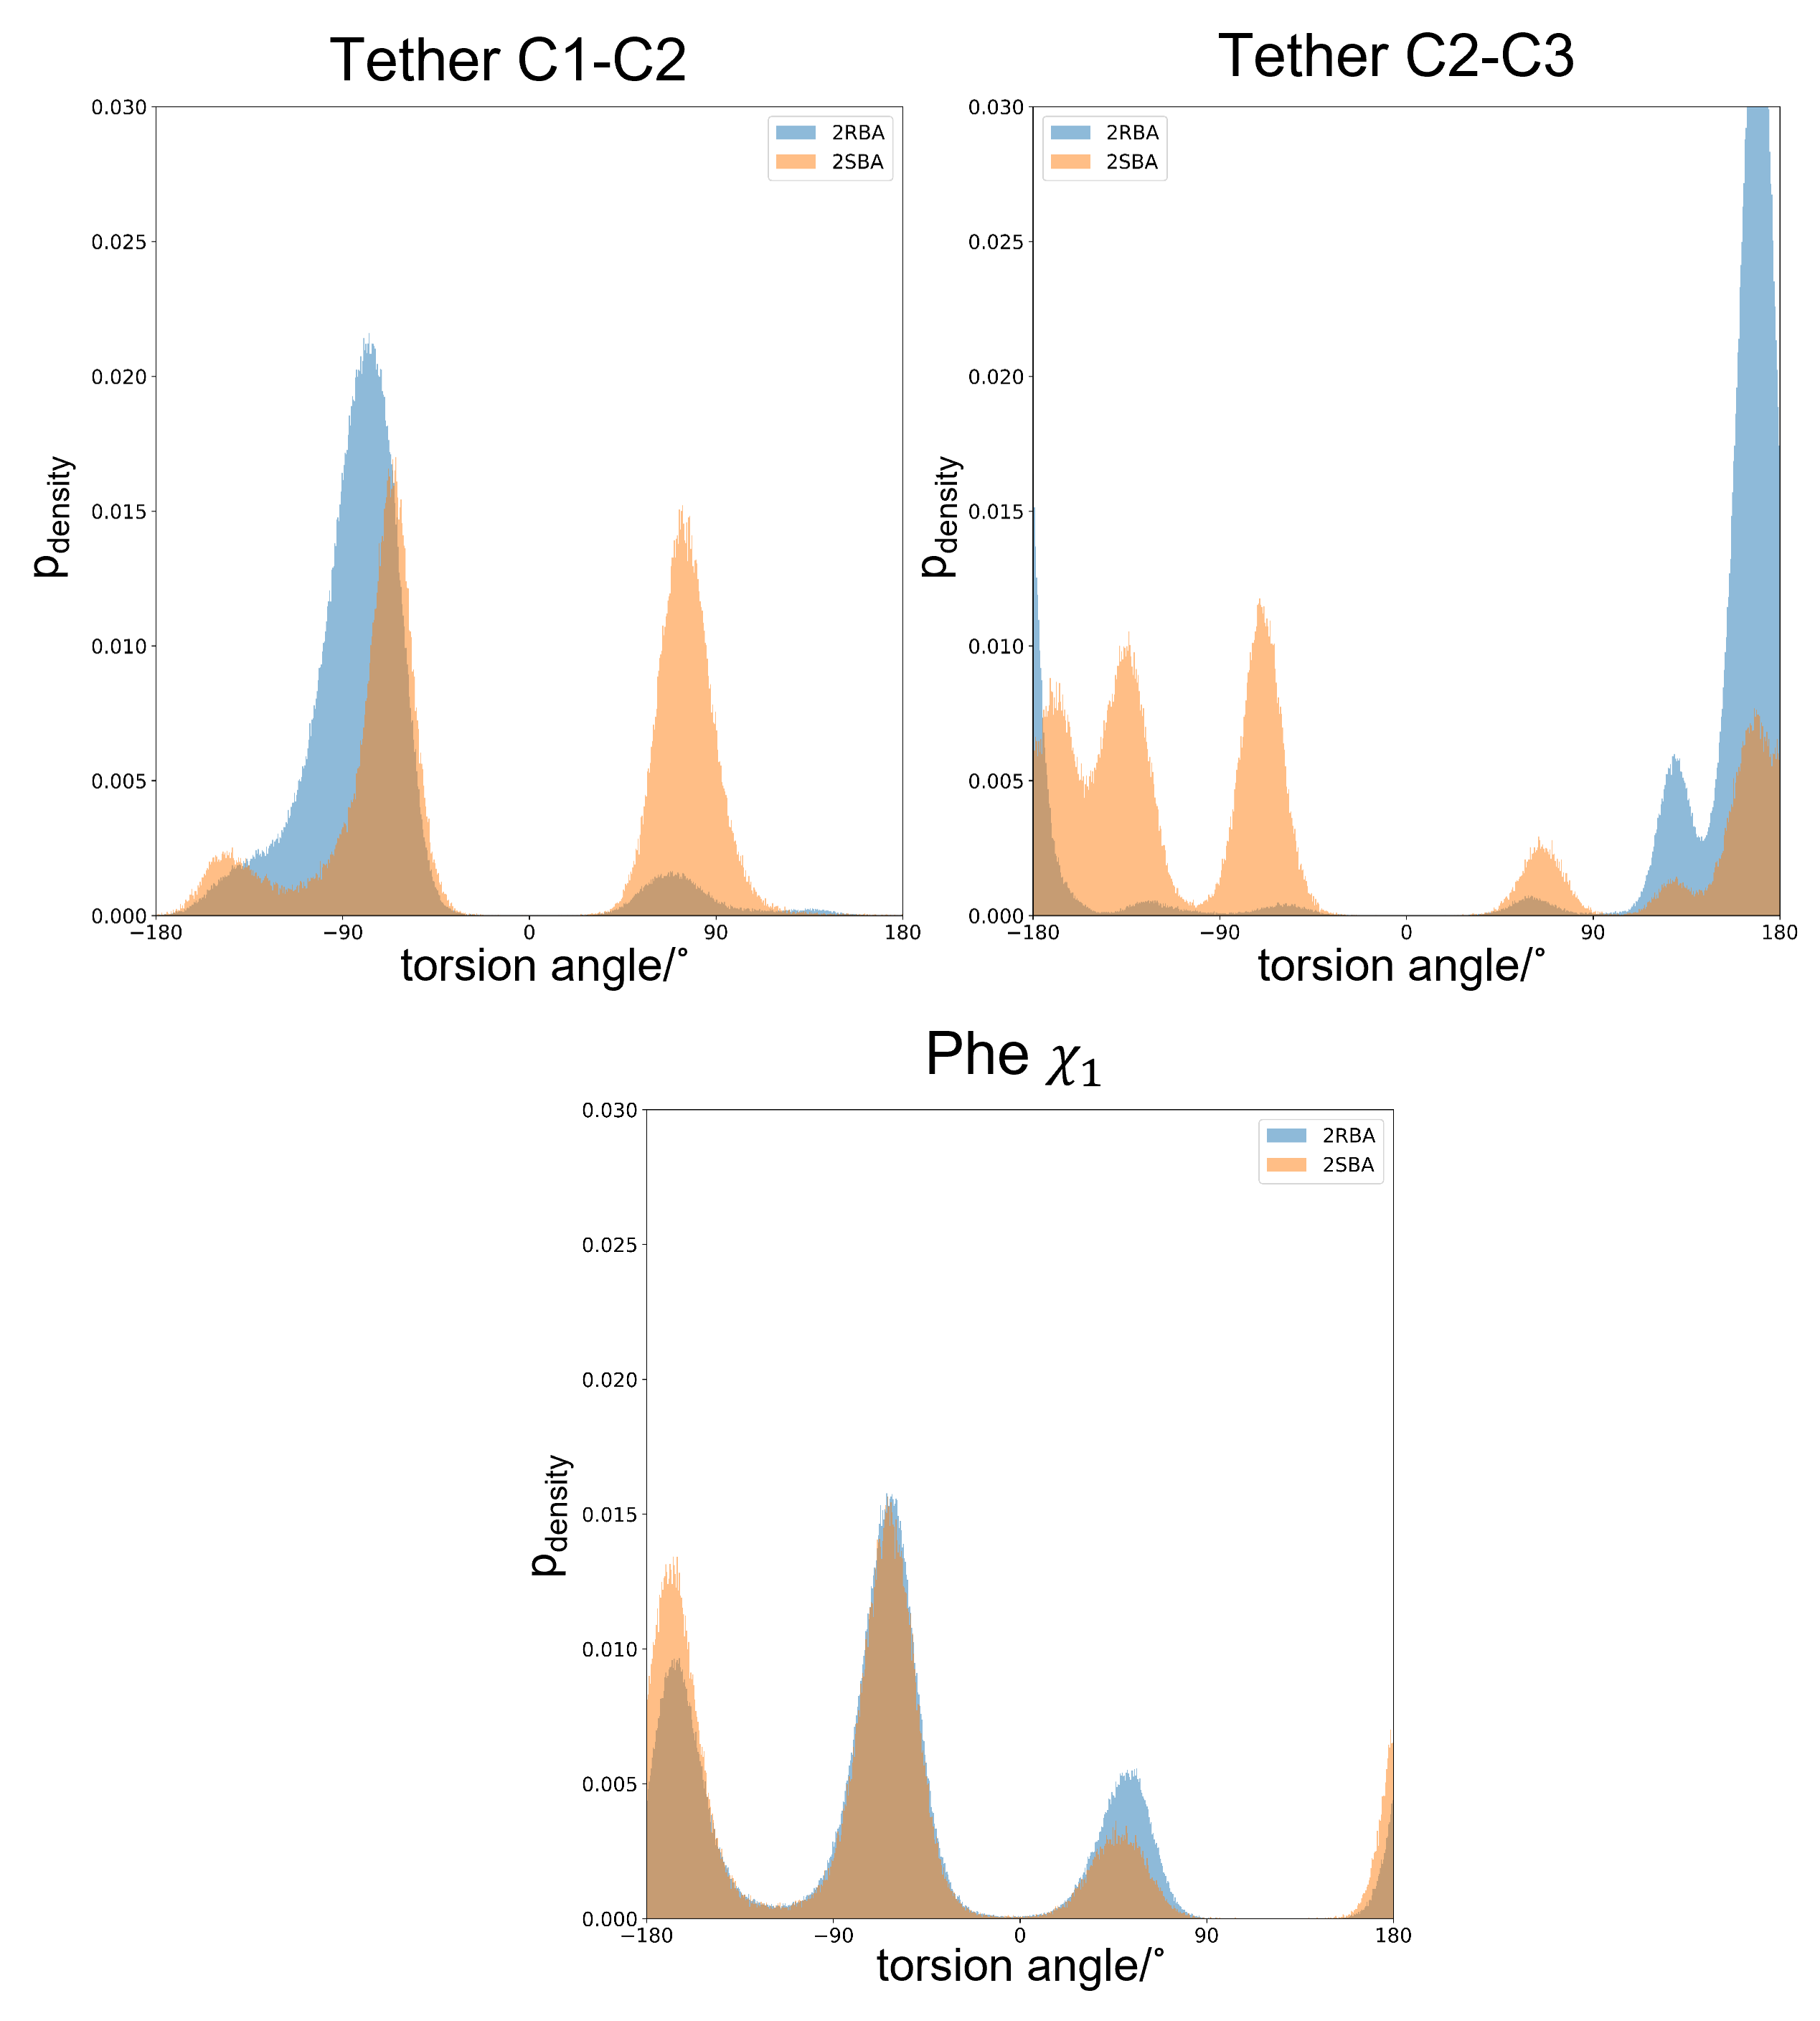
\includegraphics[width=\textwidth]{7_chapter_5/fig/results/dihedral_dist_Wat.png}
    \caption{Torsional-angle distributions of the tether in Nleu-2R (blue) and Nleu-2S  (orange)  in  chloroform.  Analysis  was  restricted  to  the clusters  with  the  trans-peptoid bond. The distribution density is plotted as a function of the torsional angle, with a bin size of $0.5~\text{deg}$}
    \label{fig: SITorsion2RS}
\end{figure}


\FloatBarrier
%-------------------------------------------

\begin{table}[h!]
    \centering
    \caption{Percentage of sampled conformations with zero, one, or two hydrogen bonds
for Nleu-5R, Nleu-5S, Nleu-2R, and Nleu-2S in water. Analysis was restricted to the
clusters with the trans-peptoid bond}
    \label{tab: hbondsratiowater}
    \begin{adjustbox}{max width=\textwidth}
    \begin{tabular}{lccc}
    number of hydrogen bonds [\%] &	0 &	1 &	2 \\
    \hline
    Nleu-5R  &	87	& 12	& 1 \\
    Nleu-5S  &	74	& 26	& 0  \\
    Nleu-2R  &	78	& 22	& 0 \\
    Nleu-2S  &	76	& 24	& 0 \\
    \hline
    \end{tabular}
    \end{adjustbox}
\end{table}

The analysis of the hydrogen-bonding patterns in water showed a significant decrease for the intramolecular hydrogen bond populations, as they competed with the intermolecular hydrogen bonds to the water. Specifically, molecule Nleu-5R has a higher percentage (about $10\%$) of conformers with no H-bonds compared to Nleu-2R, Nleu-2S, and Nleu-5S (Table \ref{tab: hbondsratiowater}). The conformations containing two intramolecular hydrogen bonds nearly vanished.
The positions of the intramolecular hydrogen bonds are mainly focused on the NLEU-O tether-NH position (Table \ref{tab: SIhbondRatiosWater}).
Nevertheless, it could be observed that the ALA-O tether-NH, which was unique to the Nleu-5S in the apolar environment, is again most present in water for Nleu-5S in contrast to the other possible intramolecular hydrogen-bonds. 


\begin{table}[h!]
\centering
\caption{Hydrogen bond occurrence in percentage for the sampled conformations in
water for Nleu-5R, Nleu-5S, Nleu-2R, and Nleu-2S. The analysis was restricted to the
clusters with the trans-peptoid bond.}
\label{tab: SIhbondRatiosWater}
  \begin{adjustbox}{max width=\textwidth}
  \begin{tabular}{lcccc}
Hydrogen bond {[}\%{]} & Nleu-2R      & Nleu-2S      & Nleu-5R      & Nleu-5S      \\
\hline
NLEU-O tether-NH       & 14.5       & 18.3       &  12           & 9.75        \\
ALA-O tether-NH        & 5.5        & 3.6        & \textless{}1  & 15.25 \\
PHE-O Ala-NH           & \textless{}1 & \textless{}1 & \textless{}1  & 1 \\
ALA-O PHE-NH           & 2            & 1            & \textless{}1  & \textless{}1 \\
    \hline
\end{tabular}%
\end{adjustbox}
\end{table}

In general, however, no significant differences between the peptides could be observed in water.



\FloatBarrier
%-------------------------------------------

The findings, taken together, suggest that the permeability cliff observed between Nleu-5R and Nleu-5S is related to their propensity for conformations with a maximized number of intramolecular H-bonds in the apolar environment. Their ability to adopt such conformations is in turn affected by the stereochemistry of the methyl group at position $5$ in the tether as it determines the preferred torsional angles of the tether.

